\label{sec:newInt}
In this section, the results of the analysis are studied further. First a more detailed investigation of the properties of the excess at low \mll is conducted. Afterwards, the implications of these results on the  simplified models discussed in section~\ref{sec:models} are examined.
\section{Investigating the excess in the low-mass central region}
While a significance of $2.2\sigma$ is no clear indication for the presence of new physics, more detailed studies of the properties of this excess are conducted. 

The development of the excess during the data taking period in 2012 is shown on the left side of Figure~\ref{fig:timeDependece}, while the right side shows the low-mass forward region for comparison. The data sample is split into 10 bins, each corresponding to 2\,$\mathrm{fb}^{-1}$ within 1\%, except for the last which corresponds to only  about 1.5\,$\mathrm{fb}^{-1}$. For each of these bins the observed SF yield and the prediction for flavour-symmetric backgrounds from OF is shown, together with the difference of the two. The very small contribution from Drell--Yan backgrounds of typically less than 1 event per bin is neglected in this representation of the result. For the first four bins, corresponding to the first 8\,$\mathrm{fb}^{-1}$ of data collected in 2012, the SF yield is significantly higher than the prediction from OF. This effect diminishes in the fifth bin, where the SF yield decreases and the prediction from OF increases. In the following five bins, representing the second half of the data sample, good agreement is observed between the observed SF yield and the prediction from OF. This change in behaviour between the two halves is caused in roughly equal proportion by a decrease in the observed SF yield and an increase in the observed OF yield per bin. No known changes in data taking conditions occurred at this time. In contrast to this observations, the SF yield and the background prediction are compatible within uncertainties for all bins in the low-mass forward region. The difference between the two therefore fluctuates around zero.

\begin{figure}[tb]
\centering
\begin{minipage}[t]{0.49\textwidth}
  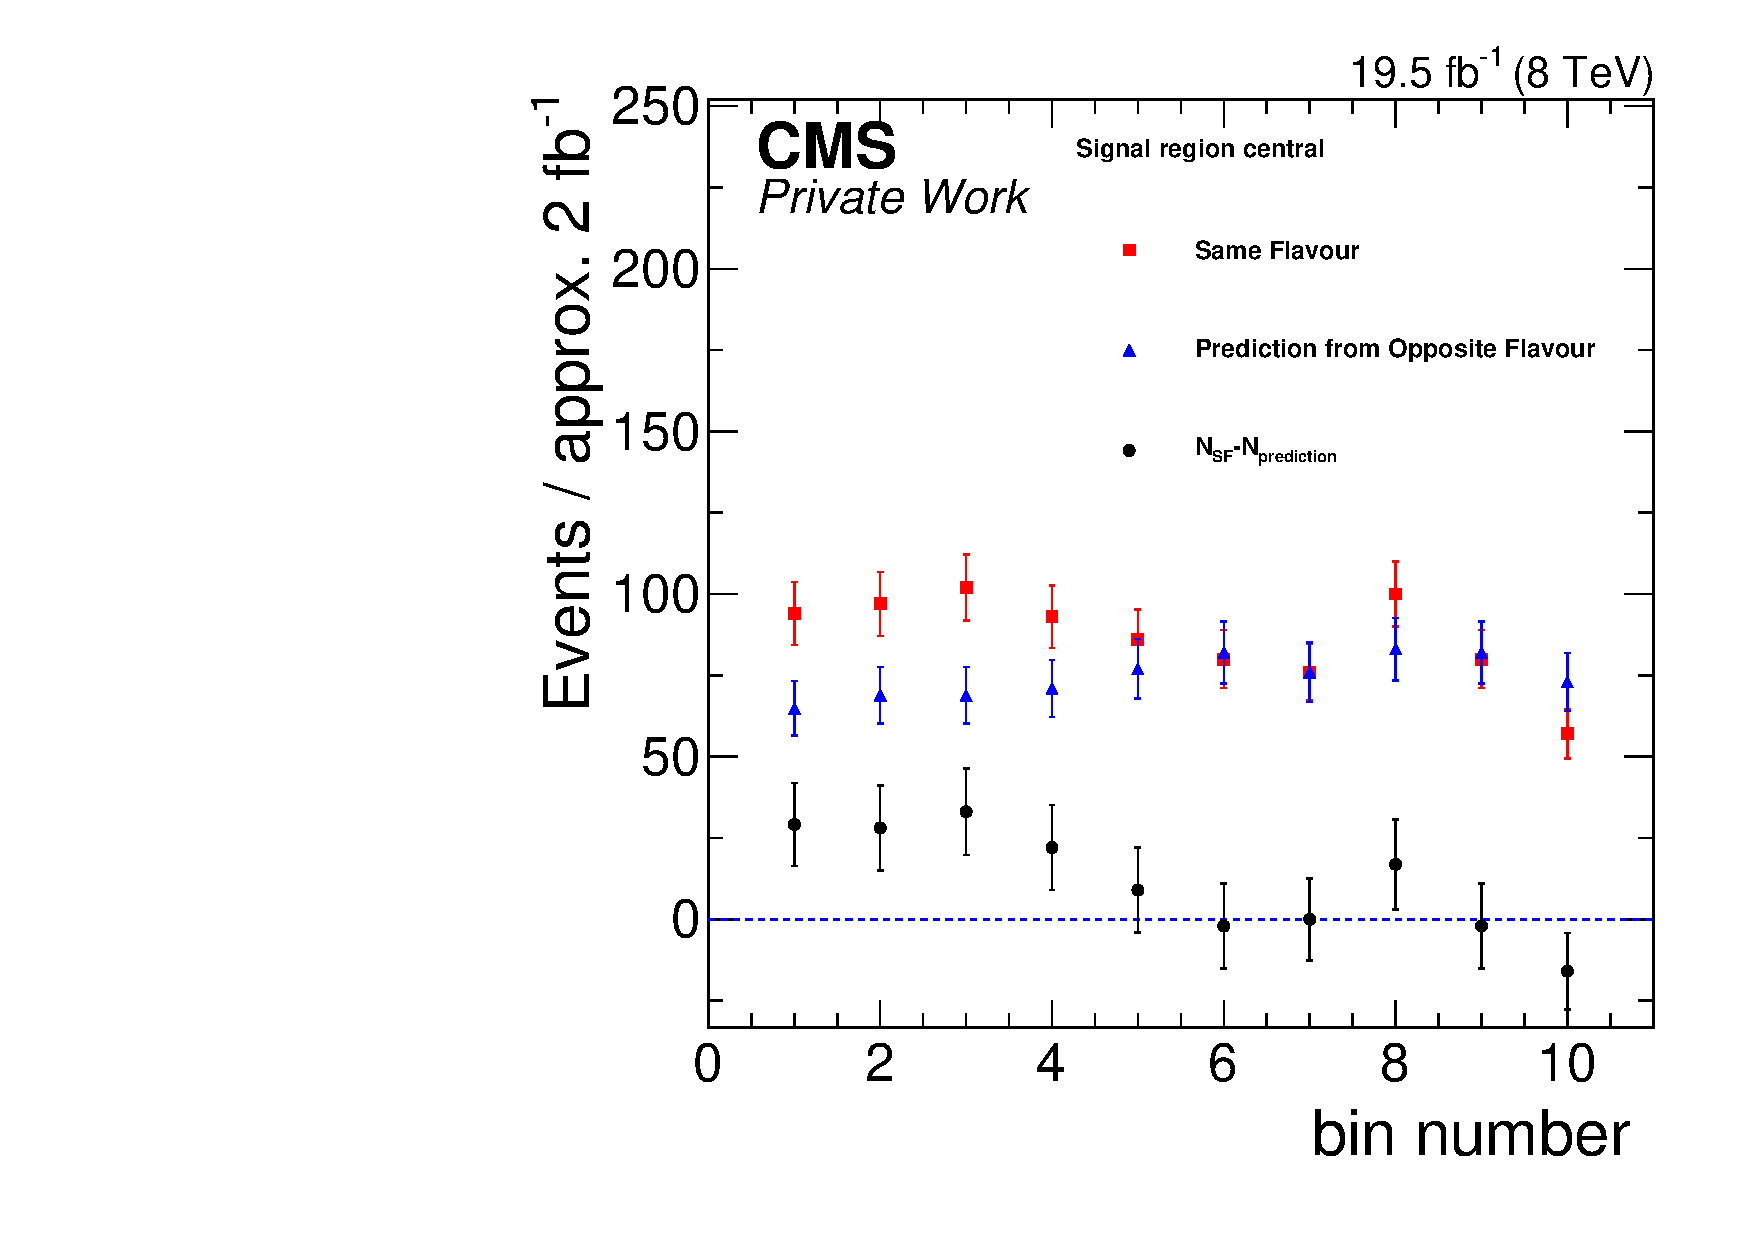
\includegraphics[width=\textwidth]{plots/results/YieldvsLumi_Bins_SignalCentral_Mll_edgeMassFull2012.pdf}
\end{minipage}
\begin{minipage}[t]{0.49\textwidth}
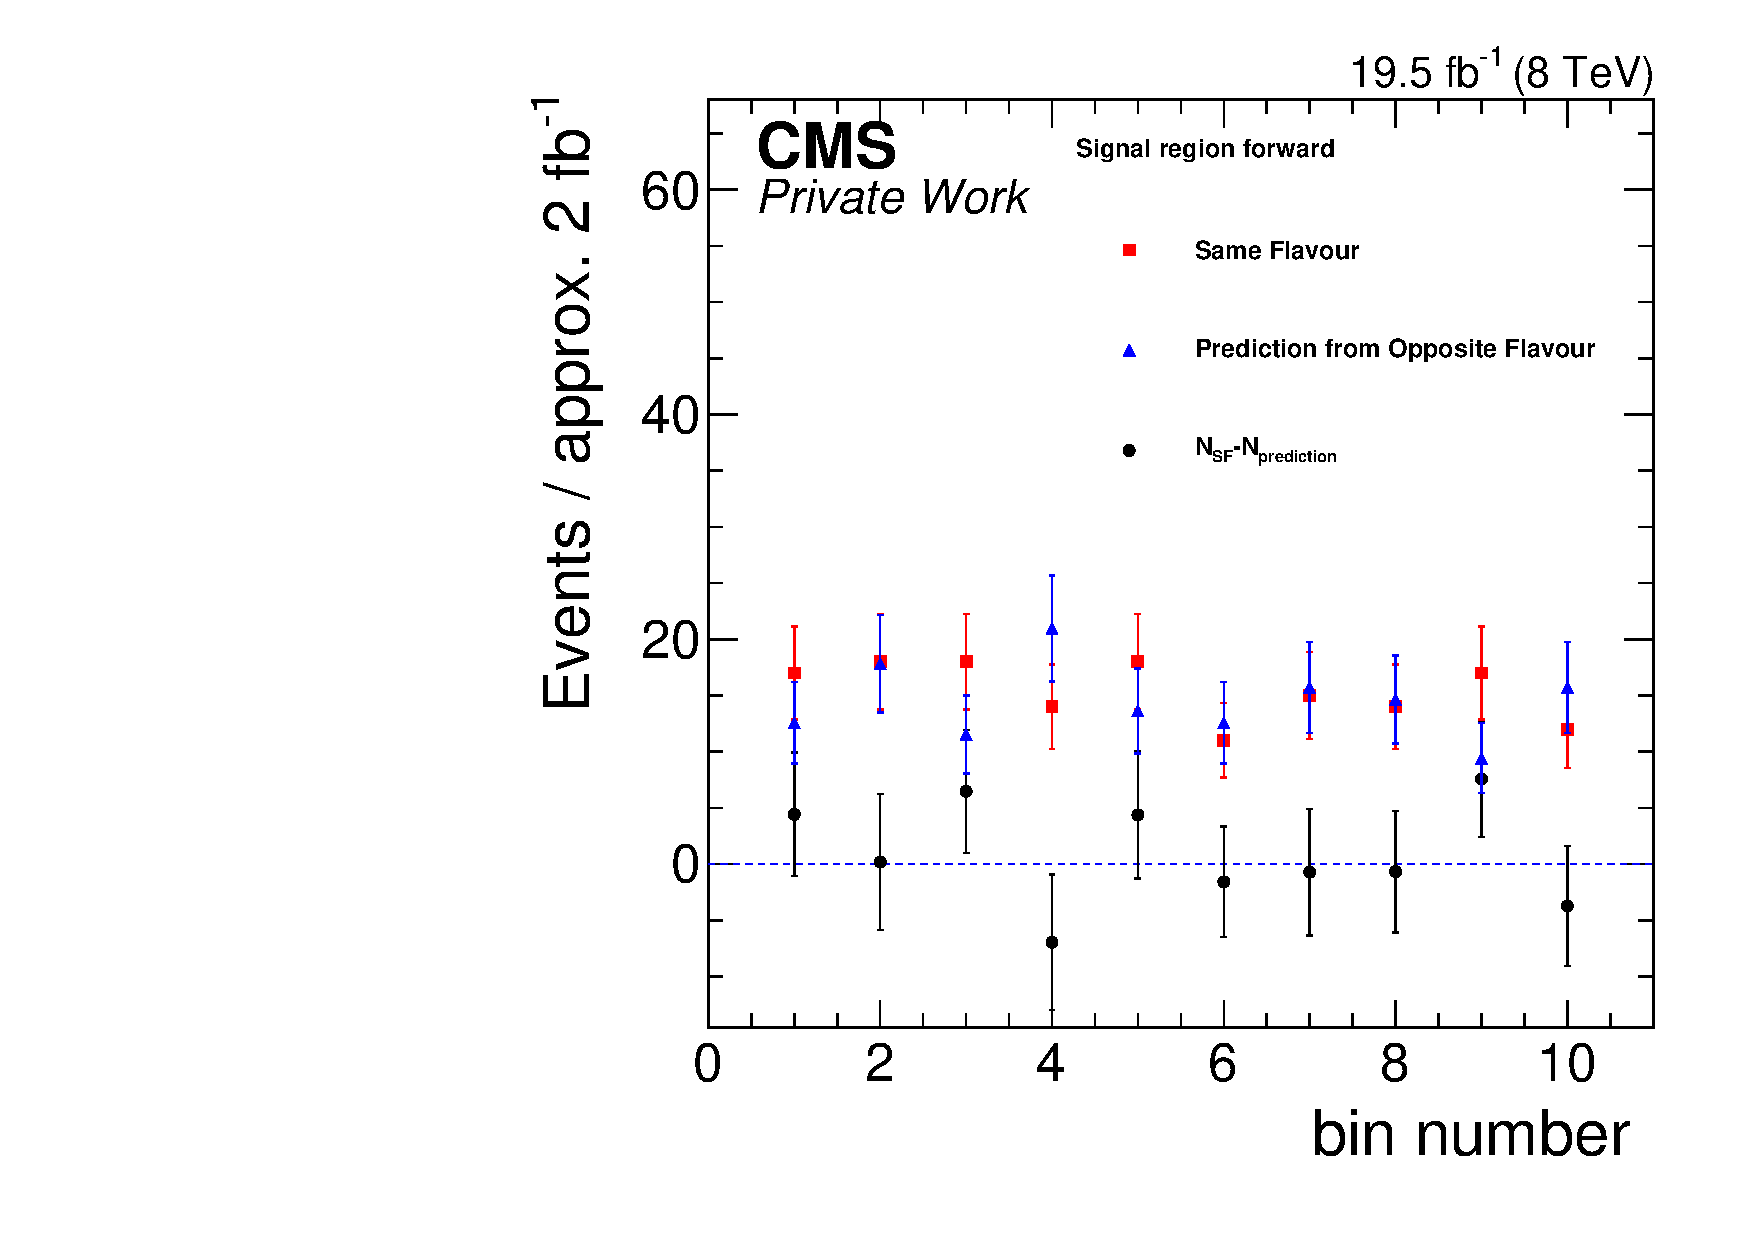
\includegraphics[width=\textwidth]{plots/results/YieldvsLumi_Bins_SignalForward_Mll_edgeMassFull2012.pdf}
\end{minipage}

\caption{Observed SF yields and background prediction from OF as well as the difference of these two in the low-mass central (left) and forward (right) signal region in 10 bins of roughly equal integrated luminosity. The bins are shown in the order the data has been recorded. Non-flavour-symmetric backgrounds are not included in this representation of the result.}
\label{fig:timeDependece}
\end{figure}

To get a clearer picture of the properties of the excess and also to check for some of the more obvious possible systematic effects that might cause it, the counting experiment in the low-mass central region is repeated several times, varying the selection requirements. As discussed in Section~\ref{sec:eventsel}, the event selection has not been changed significantly after the excess has been observed and in particular had been defined before the studies presented here were performed. The results are shown in Table~\ref{tab:CountingCrosschecks}. As no Drell-Yan prediction for the on-\Z region is available for the different selection configurations, the observed yield in the on-Z region is extrapolated into the low-mass region after subtraction of flavour-symmetric background using the prediction from OF. For the background prediction from OF the \Rsfof factor derived for the default selection is used in all these cross-checks presented here.

As the dominant $t\bar{t}$ background in the signal region produces b-tagged jets, it seems natural to test the excess for its b-tag content. Splitting the data sample into events with at least one and events without a b-tag, it is evident that, while about 23\% of all events contain no b-tagged jets, less than 10\% of the excess is located in this category. Comparing the yields of events with at least one and at least two b-tagged jets, the ratio between the two subsamples is about 2.4 for both the flavour-symmetric backgrounds and the signal. 

In addition to the default selection of $\pt > \unit{20}{\giga\electronvolt}$, four other configurations for the lepton transverse momentum requirement are tested. Three of them feature asymmetric cuts on the \pt of the leading and trailing lepton. The selection of $\pt > 20(10)\GeV$ and $ \pt > 30(10)\GeV$ extend the acceptance of the analysis to lower trailing lepton \pt. For both of these selections, an increased signal yield is observed. On the other hand, raising the trailing \pt threshold to 30\GeV disproportionally reduces the observed excess, retaining only about 13\% of the excess yield compared to 23\% of the overall event yield. 

Although it has already been established in Section~\ref{sec:validation} that non-prompt leptons only account for a small part of the selected data sample and are also fully flavour-symmetric, the counting experiment is repeated with significantly tighter isolation requirements. The relative isolation is required to be smaller than 5\%, reducing the size of the selected sample by about one third. The number of observed signal events is reduced by almost exactly the same amount. This further increases the confidence that the observed effect is due to prompt lepton production.

To test for a possible pileup dependence of the observed effect, the sample is split into three subsets of similar size depending on the number of reconstructed vertices ($N_{\mathrm{Vertex}}$). The events are categorised as either low-pileup ($N_{\mathrm{Vertex}} < $13), medium-pileup (13 $\leq N_{\mathrm{Vertex}} <$ 17) or high-pileup ($N_{\mathrm{Vertex}} \geq $17). The excess is observed consistently in all three subsets, excluding a possible pileup dependence of the excess. 

Three additional \MET reconstruction algorithms are tested. Track-corrected (TC) \MET and type-I corrected PF \MET have been described in Section~\ref{sec:PF}. In addition to these general algorithms, an analysis-specific definition of missing $H_{\mathrm{T}}$ is used, which is calculated using only selected jets and leptons. It is defined as the absolute value of the negative vector sum of the transverse momenta of these objects: 
\begin{equation*}
H_{\mathrm{T}}^{\mathrm{miss}} = \abs{ -\left(\sum\limits_{\mathrm{jets}}\vec{p}_{\mathrm{T}} + \sum\limits_{\mathrm{leptons}}\vec{p}_{\mathrm{T}}\right) }.
\end{equation*}
The signal region requirements of $\unit{100}{\giga\electronvolt}$ and $\unit{150}{\giga\electronvolt}$, depending on \njets, are applied for each of these \MET values.  Both the use of type-I corrected PF \MET and missing $H_{\mathrm{T}}$ lead to higher event yields in the signal region. Judging by the size of the Drell--Yan background, TC \MET and $H_{\mathrm{T}}^{\mathrm{miss}}$ have significantly worse \MET resolution compared to both types of PF \MET. The excess is present in all three cases and is therefore not likely to be caused by a faulty \MET reconstruction. 

Separating the data sample into events with low \HT ($\unit{100}{\giga\electronvolt} < \HT <\unit{300}{\giga\electronvolt}$) and high \HT ($\HT > \unit{300}{\giga\electronvolt}$) creates two subsets of roughly the same size. The excess is present in both subsets with similar strength. 
 


\begin{table}[hbtp]
 \renewcommand{\arraystretch}{1.3}
 \setlength{\belowcaptionskip}{6pt}
 \centering
 \caption{Results of the counting experiment in the low-mass central signal region for different variations of the event selection. The observed event yield in SF events is compared with the combined estimate from flavour-symmetric and Drell--Yan backgrounds. The estimate for the Drell--Yan backgrounds is obtained by extrapolating the event yield in the on-Z signal region after subtraction of flavour-symmetric backgrounds to the low-mass region using the \Routin factor.}
  \label{tab:CountingCrosschecks}
  \begin{tabular}{l|c|c|c|c}
                                &  SF        & Flavour-symmetric  &  Drell--Yan  & Observed - Estimates \\ 

    \hline
    \hline
 & \multicolumn{4}{c}{b-tagging}\\ 
\hline 
        no b-tags       &  202                   & 188.5$\pm$15.4              &  7.1$\pm$2.5            &  6.3$\pm$21.1 \\
        $\geq$ 1 b-tags       &  663                   & 558.4$\pm$31.0              &  1.9$\pm$0.7            &  102.7$\pm$40.3 \\
\hline 
 & \multicolumn{4}{c}{lepton \pt requirement} \\ 
\hline 
        \pt > 20(10)\GeV       &  1474                   & 1290.2$\pm$58.6              &  11.4$\pm$4.1            &  172.5$\pm$70.1 \\
        \pt > 30(10)\GeV       &  1262                   & 1114.8$\pm$52.1              &  11.3$\pm$4.1            &  135.9$\pm$63.2 \\
        \pt > 30(20)\GeV       &  761                   & 674.0$\pm$35.5              &  9.0$\pm$3.3            &  78.0$\pm$45.1 \\
        \pt > 30\GeV       &  296                   & 275.7$\pm$19.4              &  6.5$\pm$2.3            &  13.8$\pm$26.0 \\
\hline 
 & \multicolumn{4}{c}{tight lepton isolation} \\ 
\hline 
        rel. isolation < 0.05       &  572                   & 491.5$\pm$28.4              &  7.1$\pm$2.6            &  73.3$\pm$37.2 \\
\hline 
 & \multicolumn{4}{c}{pileup} \\ 
\hline 
        $N_{\text{vtx}} <$ 13       &  332                   & 289.9$\pm$20.0              &  3.3$\pm$1.2            &  38.8$\pm$27.1 \\
        13 $\leq N_{\text{vtx}}$ < 17       &  242                   & 212.8$\pm$16.5              &  0.9$\pm$0.3            &  28.3$\pm$22.7 \\
        $N_{\text{vtx}} \geq$ 17       &  291                   & 244.2$\pm$18.0              &  4.8$\pm$1.7            &  41.9$\pm$24.8 \\
\hline 
 & \multicolumn{4}{c}{\MET reconstructions}\\
\hline 
        type I corrected PF \MET       &  1034                   & 923.3$\pm$45.0              &  9.4$\pm$3.4            &  101.3$\pm$55.4 \\
        track corrected \MET       &  850                   & 702.3$\pm$36.6              &  26.3$\pm$9.4            &  121.3$\pm$47.7 \\
        missing $H_{\mathrm{T}}$       &  1171                   & 942.5$\pm$45.7              &  50.8$\pm$18.1            &  177.6$\pm$59.9 \\
\hline 
 & \multicolumn{4}{c}{$H_{\mathrm{T}}$}\\
\hline 
        100\GeV $< H_{\mathrm{T}} < $ 300\GeV        &  455                   & 401.3$\pm$24.7              &  1.4$\pm$0.5            &  52.3$\pm$32.7 \\
        $H_{\mathrm{T}} > $ 300\GeV        &  410                   & 344.6$\pm$22.4              &  7.5$\pm$2.7            &  57.9$\pm$30.3 \\
\hline 


  \end{tabular}
\end{table}




The distributions of several observables in the low-mass central signal region are shown in Figure~\ref{fig:dependencies}. Each time the observed data are compared to the prediction from OF events. The contribution from Drell--Yan backgrounds is neglected. The excess is located predominantly in events with one or two b-tagged jets, but no excess is observed for higher b-tag multiplicities. Furthermore, it is located almost exclusively in events with three jets. It is present in events with a \pt of the leading lepton of up to $\unit{60}{\giga\electronvolt}$. For events with a trailing lepton \pt above $\unit{25}{\giga\electronvolt}$, only a small deviation from the expectation is observed. The excess seems to favour low values of \MET and is roughly uniformly distributed in \HT. 

In all performed studies, no evidence for systematic effects causing the observed excess is found. The three major distinguishing features of the events causing the deviation, in addition to their low values of \mll, are the presence of at least one b-tagged jet, a jet multiplicity of three, and trailing leptons with very low \pt. However, as the distributions of these observables are still very similar to those of the dominant \ttbar background, the excess is still consistent with a statistical fluctuations of the background. 

\begin{figure}[htbp]
\centering
\begin{minipage}[t]{0.49\textwidth}
  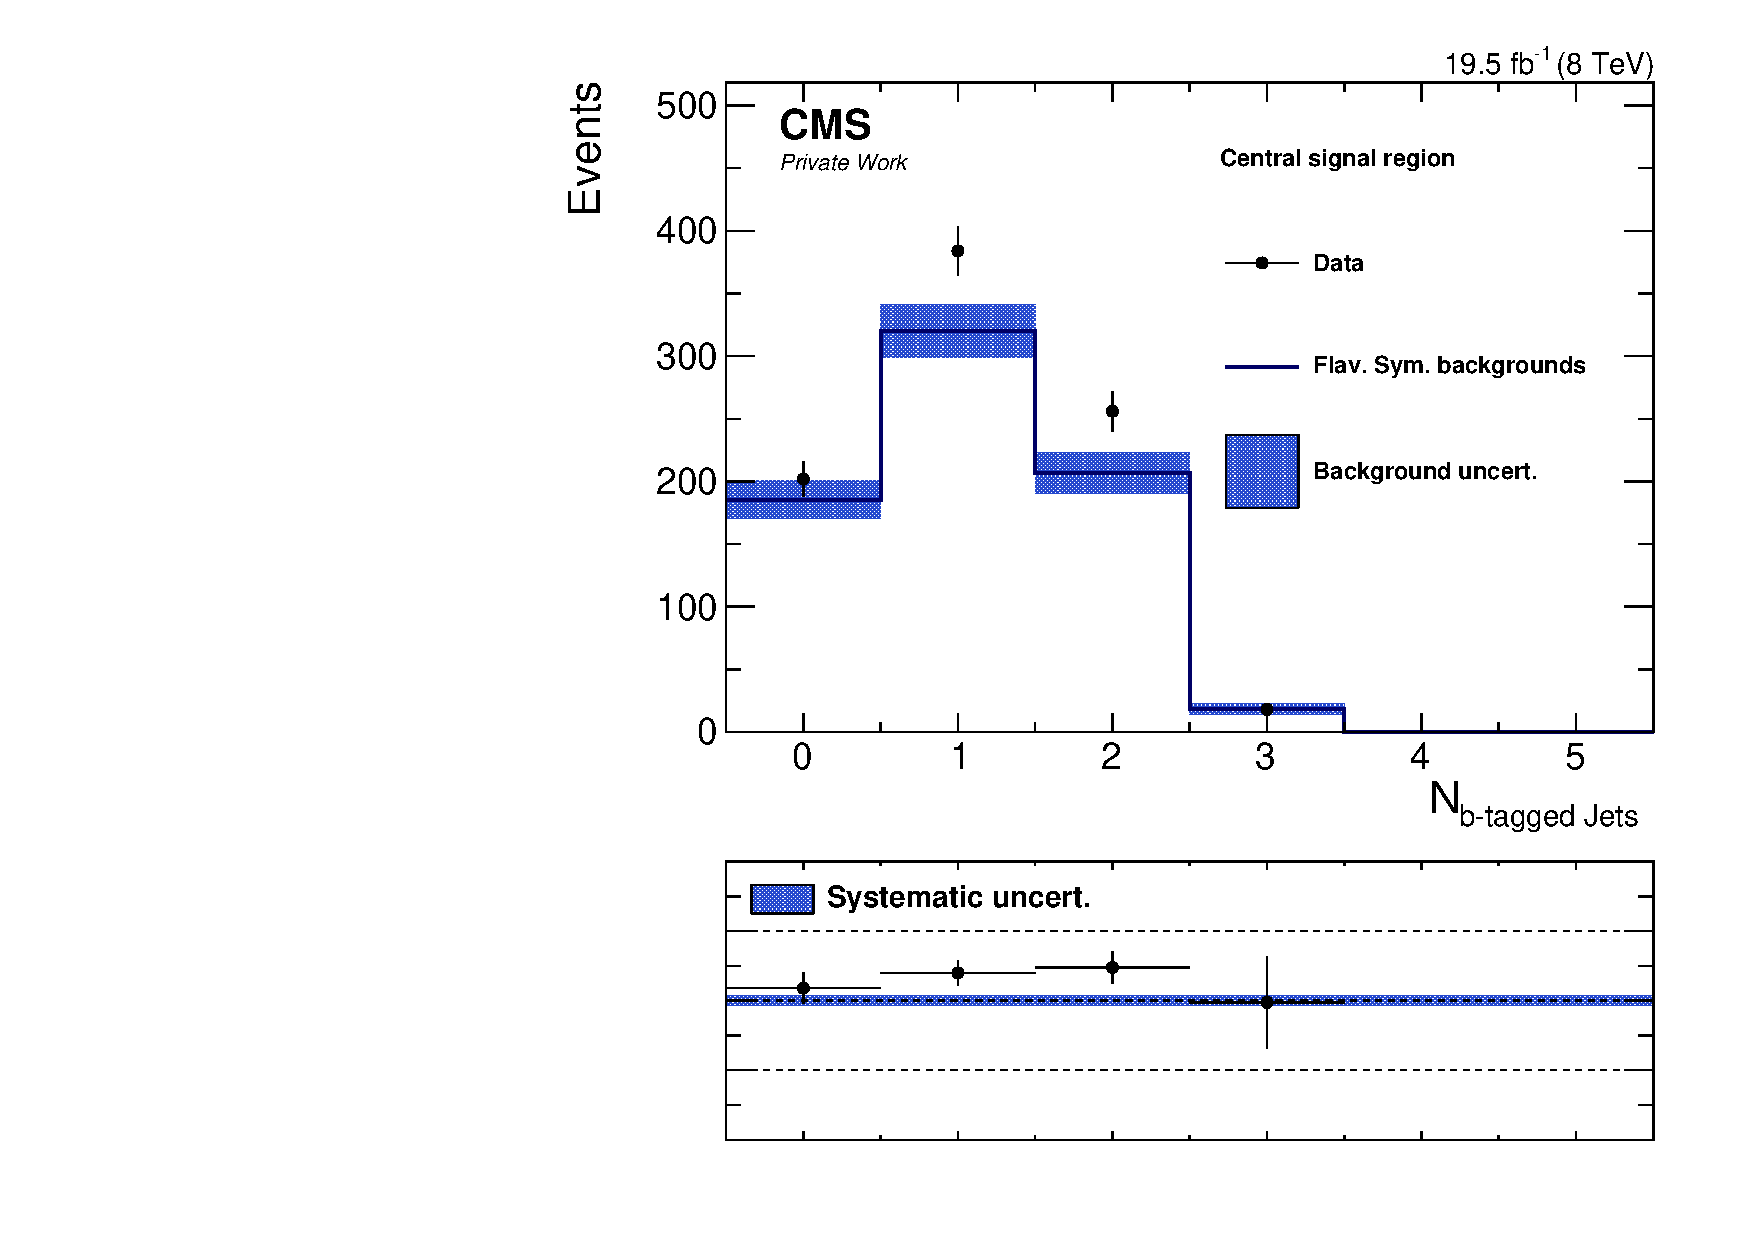
\includegraphics[width=\textwidth]{plots/results/rSFOFDependencies/rSFOFDependency_SignalCentral_NBJets_Full2012_SF_lowMass.pdf}
\end{minipage}
\begin{minipage}[t]{0.49\textwidth}
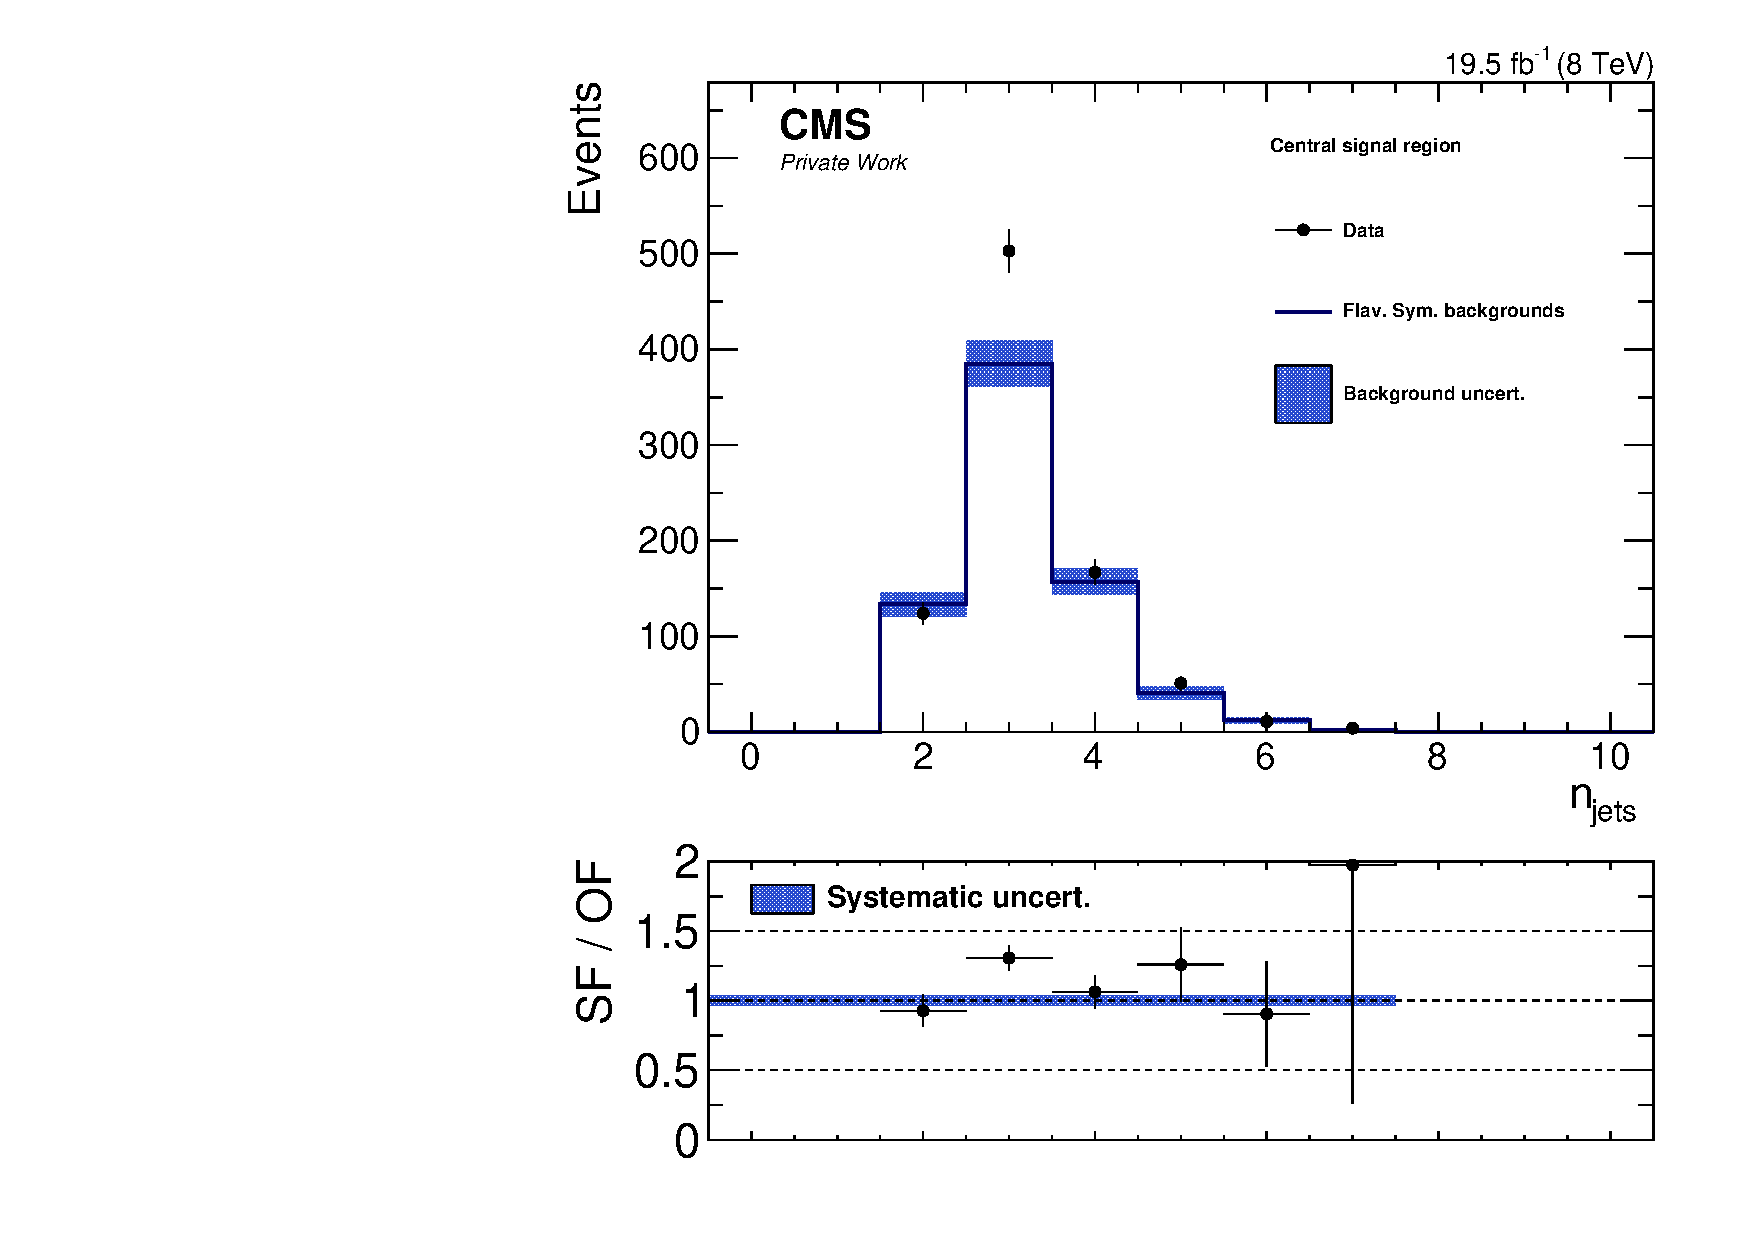
\includegraphics[width=\textwidth]{plots/results/rSFOFDependencies/rSFOFDependency_SignalCentral_NJets_Full2012_SF_lowMass.pdf}
\end{minipage}
\begin{minipage}[t]{0.49\textwidth}
  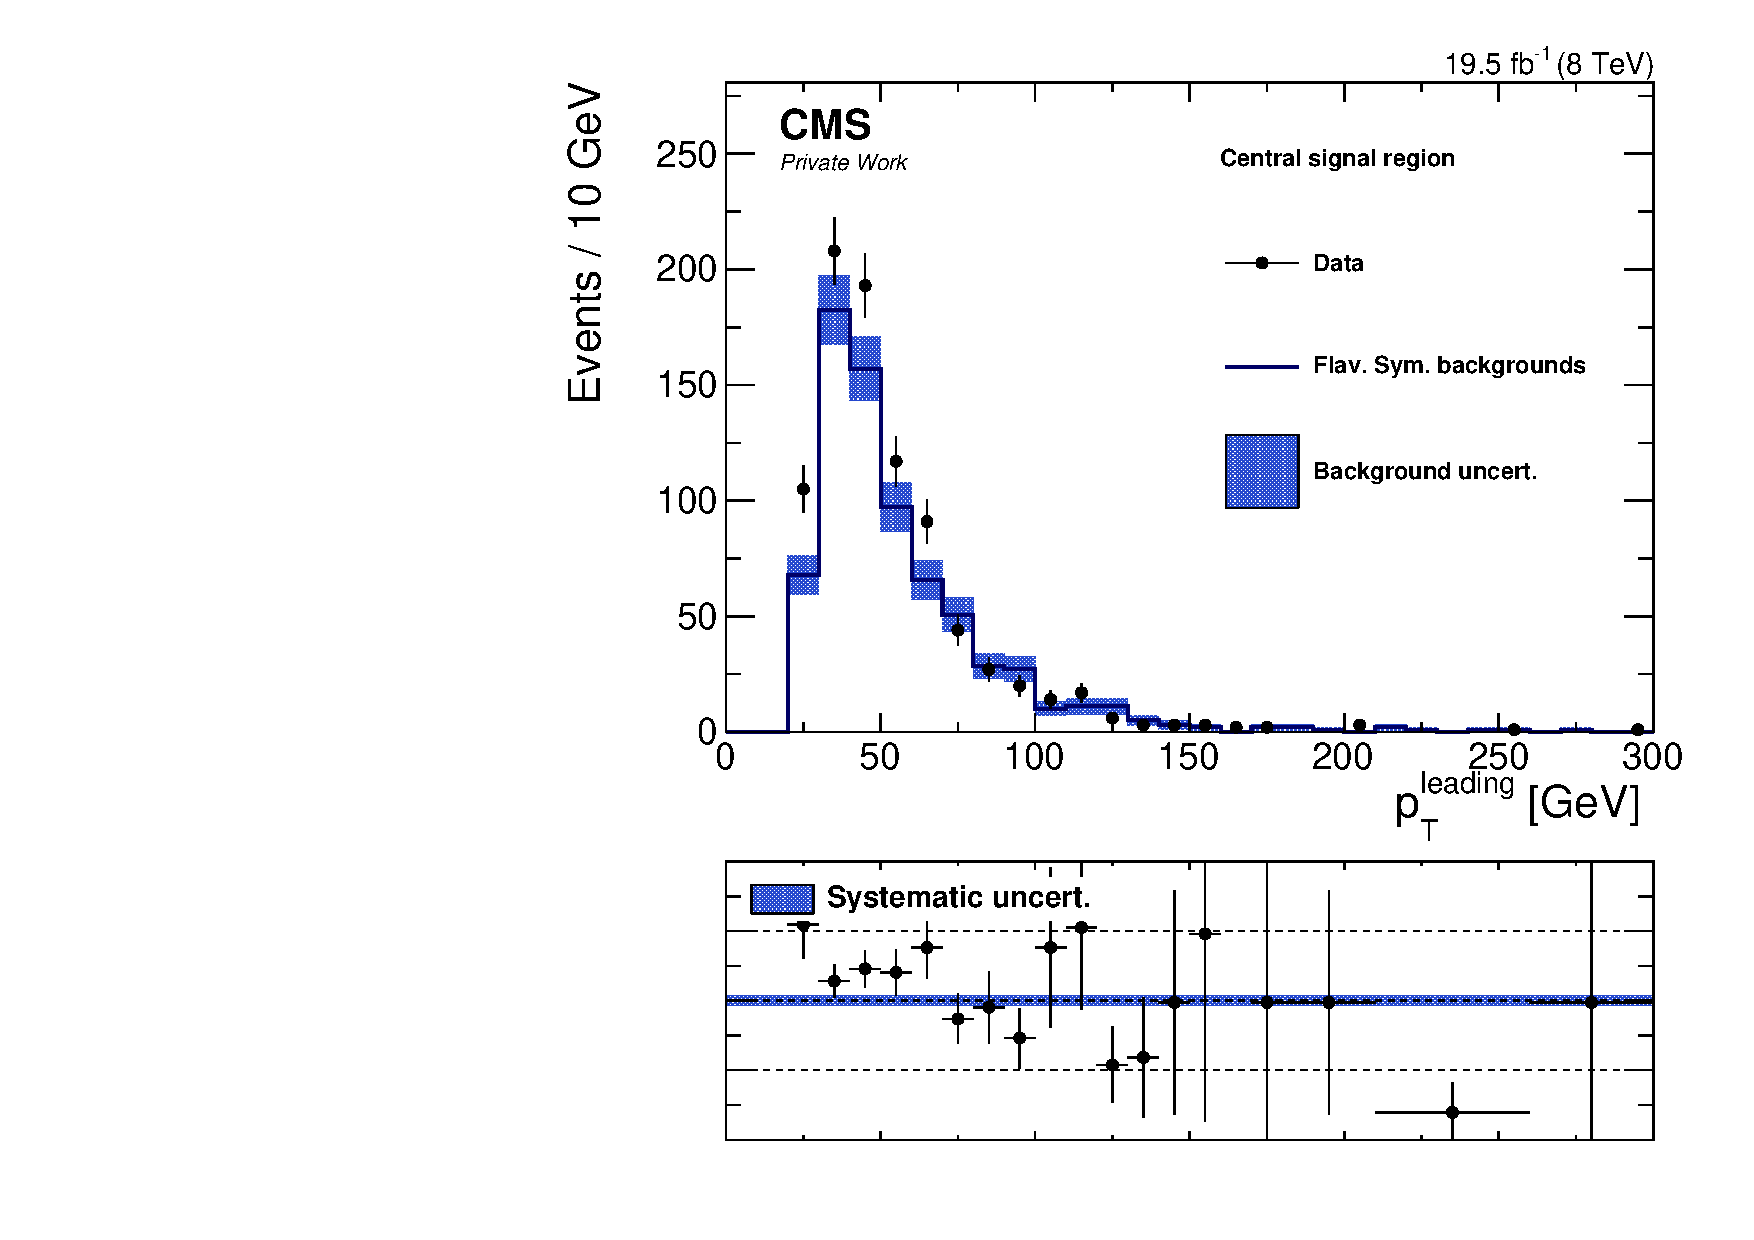
\includegraphics[width=\textwidth]{plots/results/rSFOFDependencies/rSFOFDependency_SignalCentral_LeadingPt_Full2012_SF_lowMass.pdf}
\end{minipage}
\begin{minipage}[t]{0.49\textwidth}
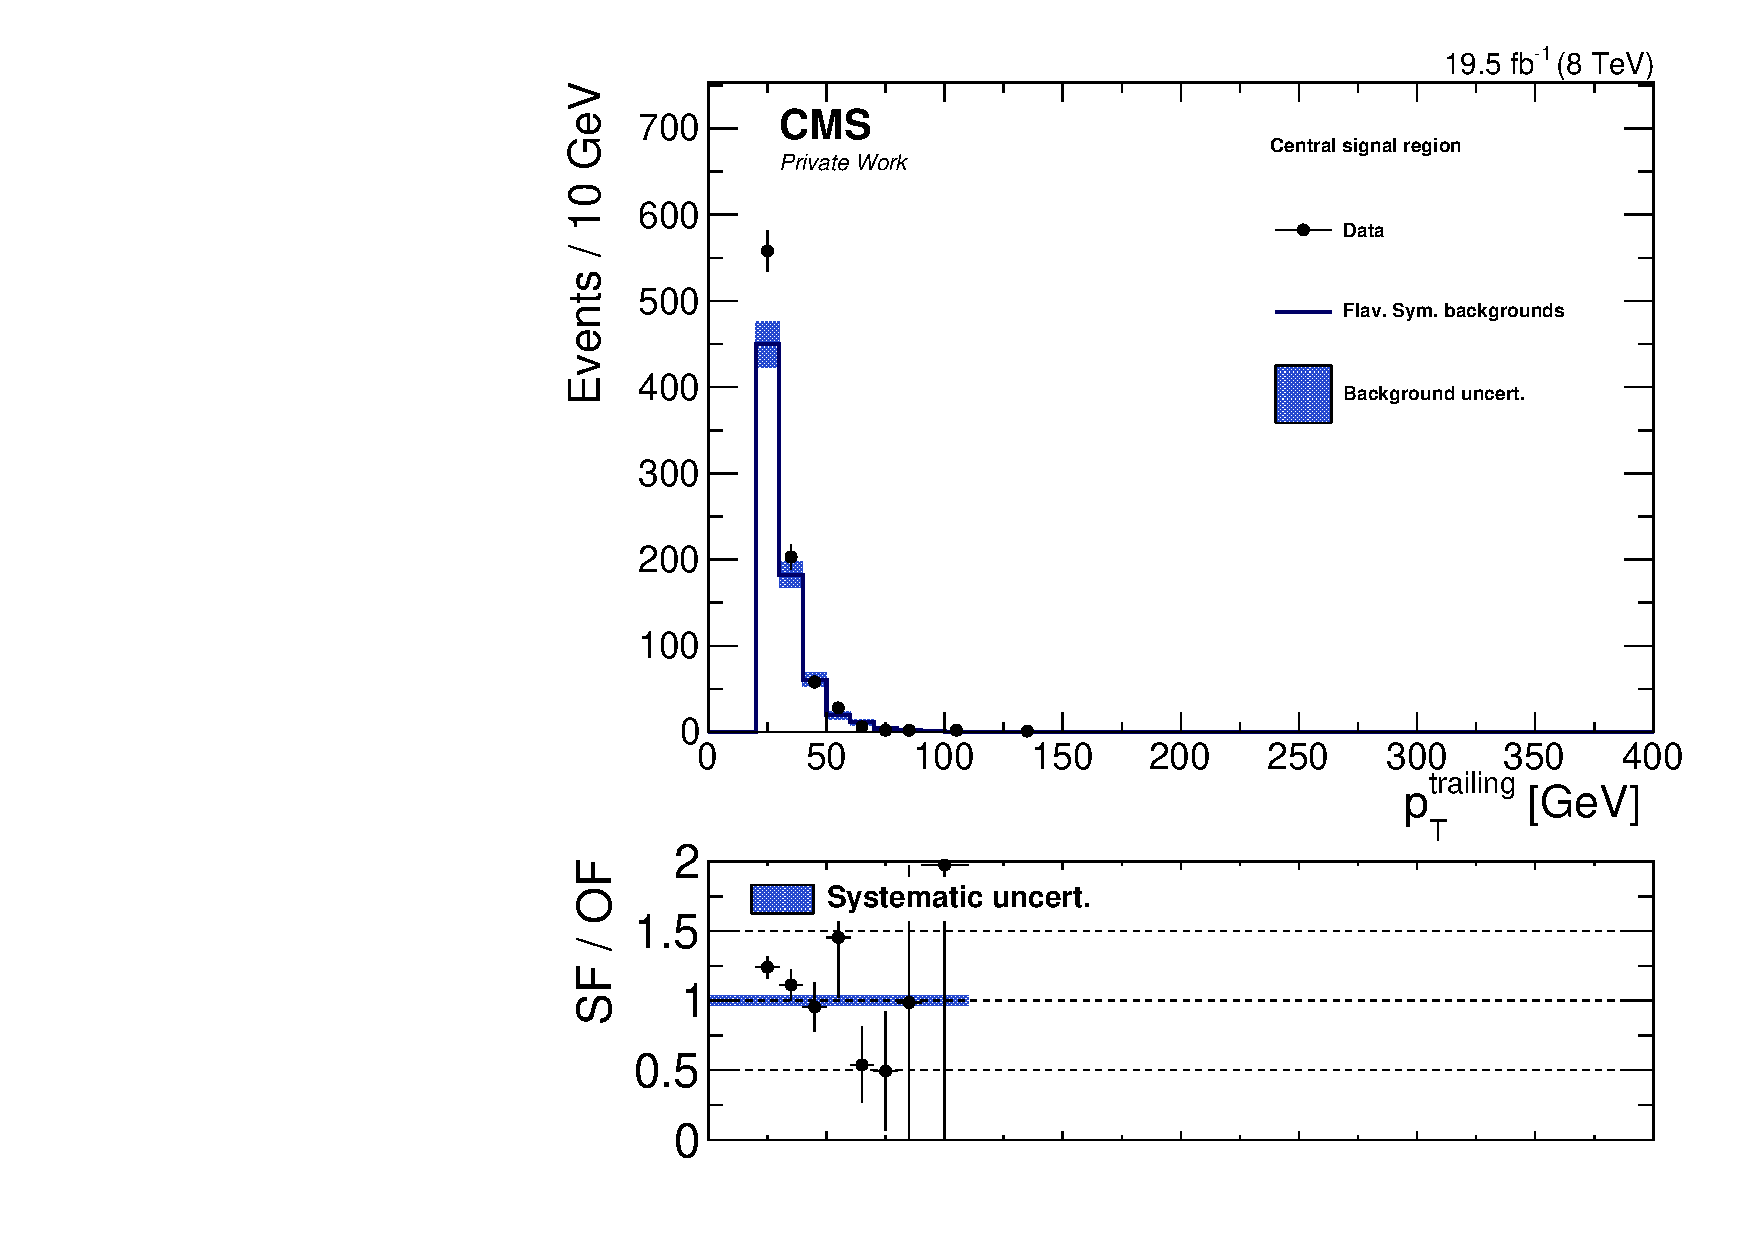
\includegraphics[width=\textwidth]{plots/results/rSFOFDependencies/rSFOFDependency_SignalCentral_TrailingPt_Full2012_SF_lowMass.pdf}
\end{minipage}
\begin{minipage}[t]{0.49\textwidth}
  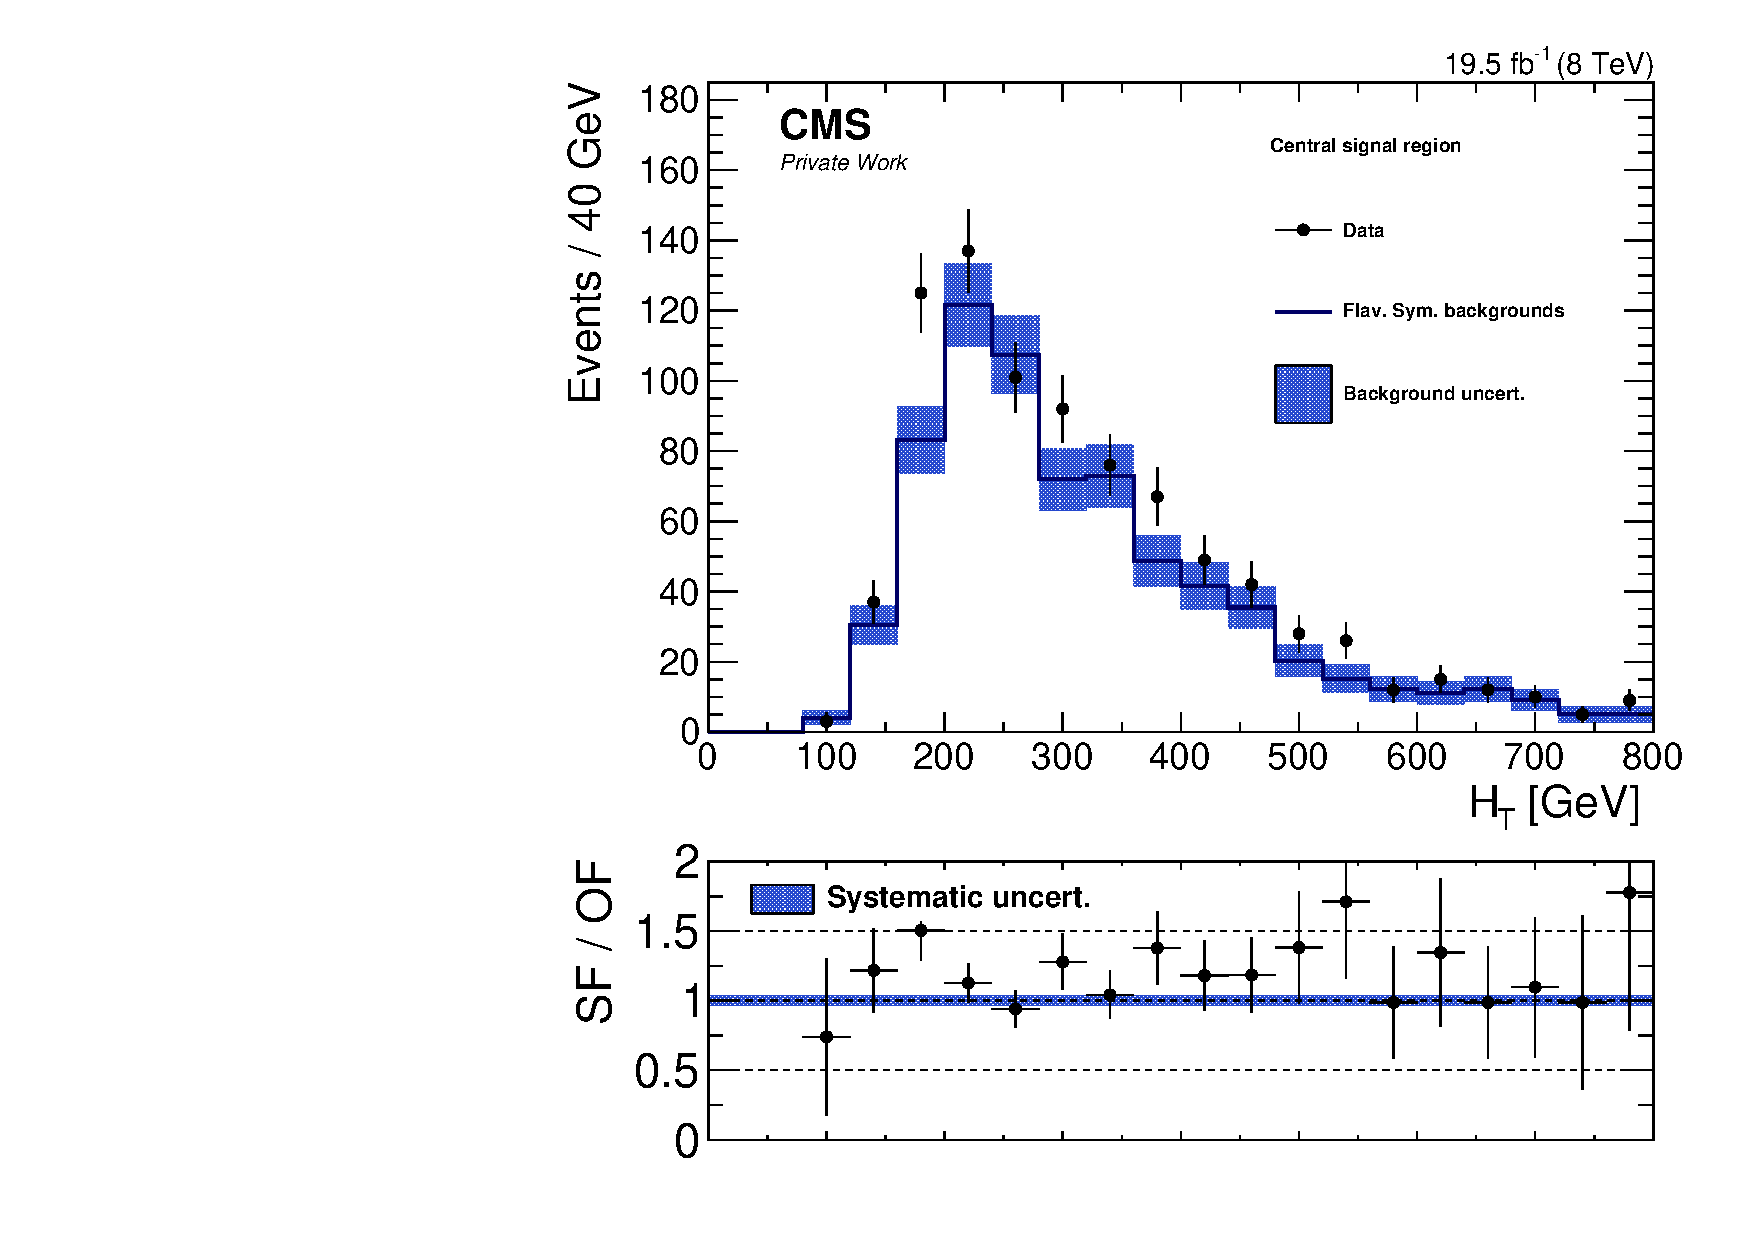
\includegraphics[width=\textwidth]{plots/results/rSFOFDependencies/rSFOFDependency_SignalCentral_HT_Full2012_SF_lowMass.pdf}
\end{minipage}
\begin{minipage}[t]{0.49\textwidth}
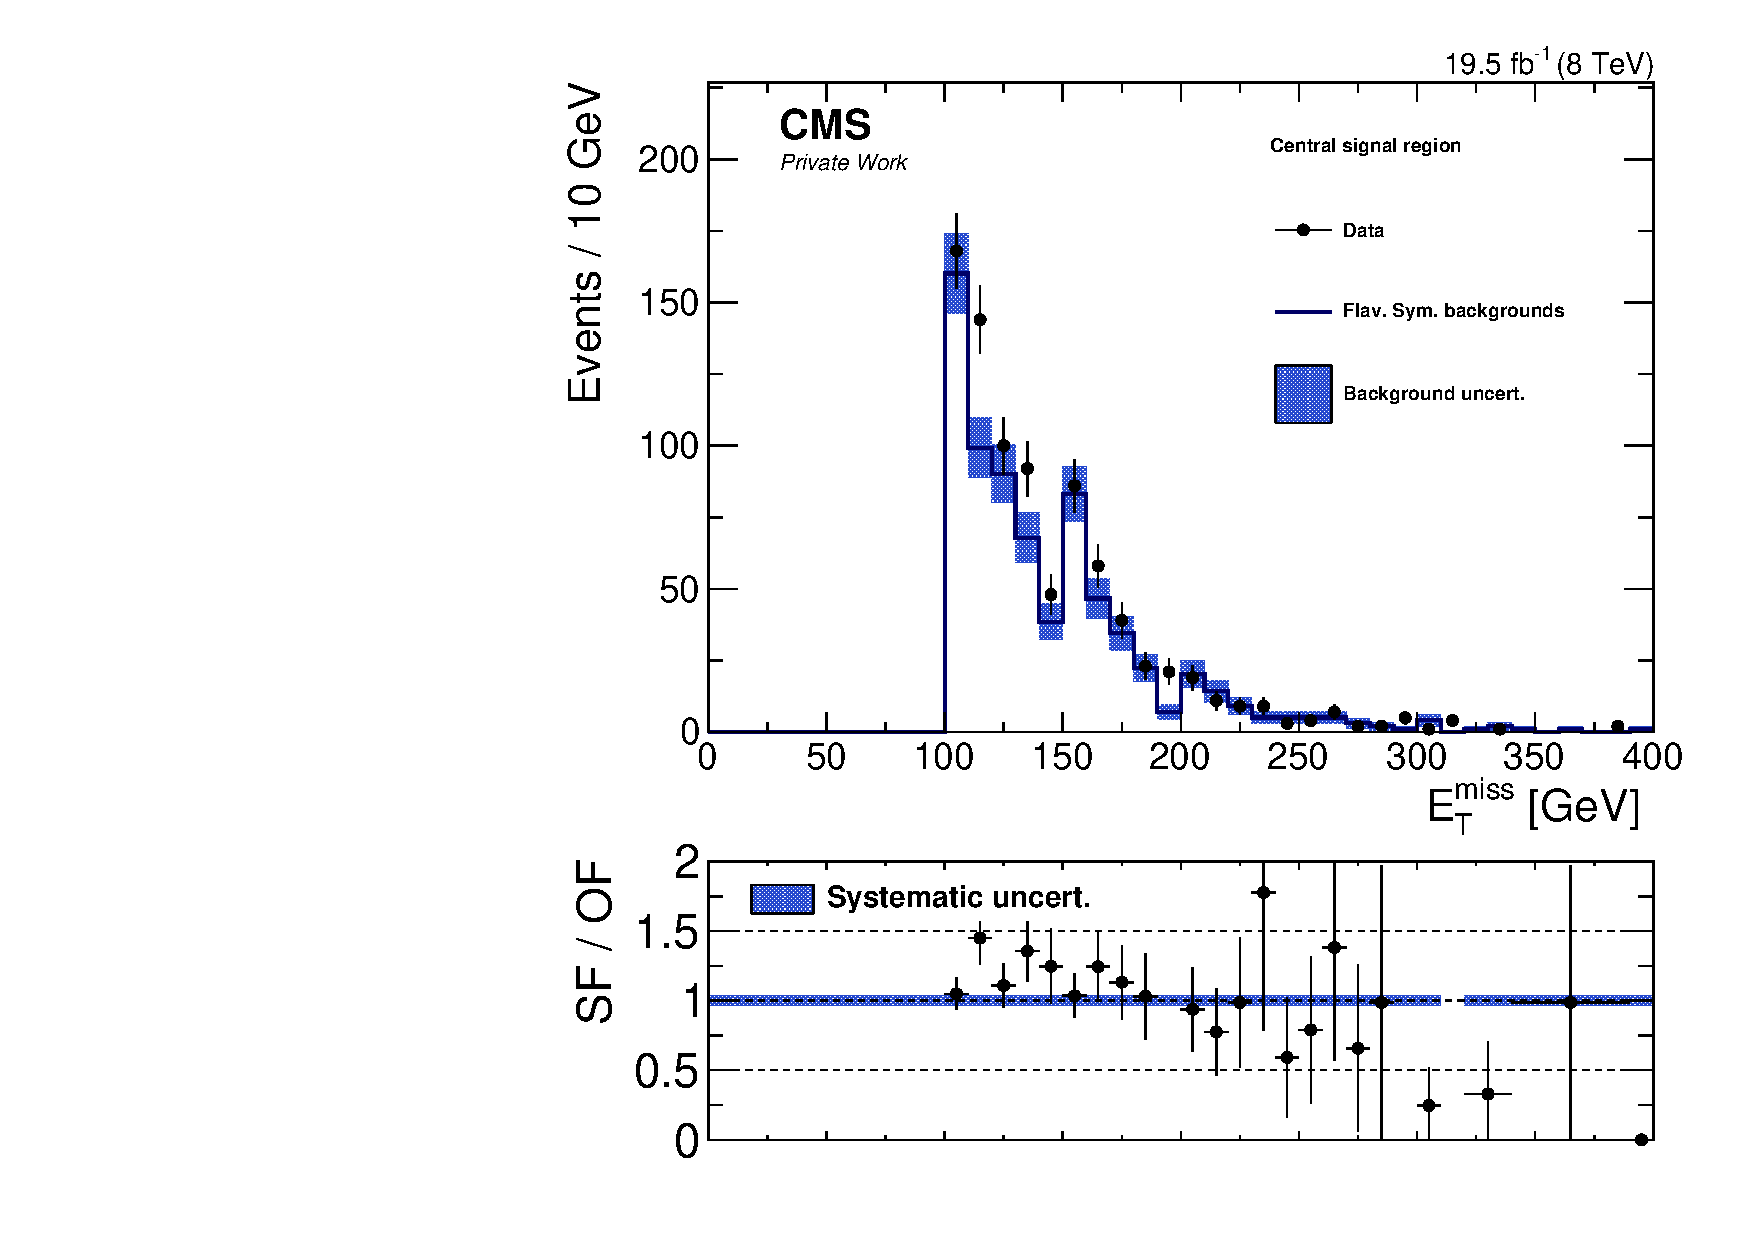
\includegraphics[width=\textwidth]{plots/results/rSFOFDependencies/rSFOFDependency_SignalCentral_MET_Full2012_SF_lowMass.pdf}
\end{minipage}
\caption{Distribution of the number of b-tagged jets (top left), jets (top right), \pt of the leading (middle left) and trailing (middle right) lepton, \HT (bottom left), and \MET (bottom right) in the low-mass central signal region. The data is shown as black dots, while the total background prediction from data is shown as a blue histogram. The blue error bars indicate the combined statistical and systematic background uncertainty in each bin. The contribution from Drell--Yan backgrounds is neglected.}
\label{fig:dependencies}
\end{figure}


\section{Interpretation in simplified models}
The absence of a clear indication for the existence of SUSY in the results of the counting experiment presented in Section~\ref{sec:candcresults} constrains the validity of supersymmetric models. To quantify the impact these results have on the allowed parameter space, they are interpreted in specific signal scenarios. Here, the two simplified models discussed in Section~\ref{sec:models} are used. 

\subsubsection{Selection efficiencies}
The impact of branching fractions, detector acceptance, and selection efficiencies on the different signal points is shown in Figure~\ref{fig:sigEff} for the example of the central signal region for the fixed-edge (left) and slepton-edge (right) models. Because of the much larger branching fraction into lepton pairs in the case of the slepton-edge model, caused by the presence of the slepton in decay chain, the overall acceptance$\times$efficiency is an order of magnitude larger in this case. As the event kinematics vary depending on the sparticle masses, the efficiency strongly depends on the position of the signal point in the $m_{\sbottom}$-$m_{\secondchi}$ plane. In general, the efficiency is low along the diagonal, where little energy is available for the decay products. Another notable feature is a decrease in efficiency around \secondchi masses of about $\unit{225}{\giga\electronvolt}$ in the case of the slepton-edge model. This is caused by the gaps in the signal acceptance between the three invariant mass regions of the counting experiment. No such effect is visible for the fixed-edge case because the signal is concentrated in the low-mass region in this model.  
\begin{figure}[htbp]
\centering
\begin{minipage}[t]{0.49\textwidth}
  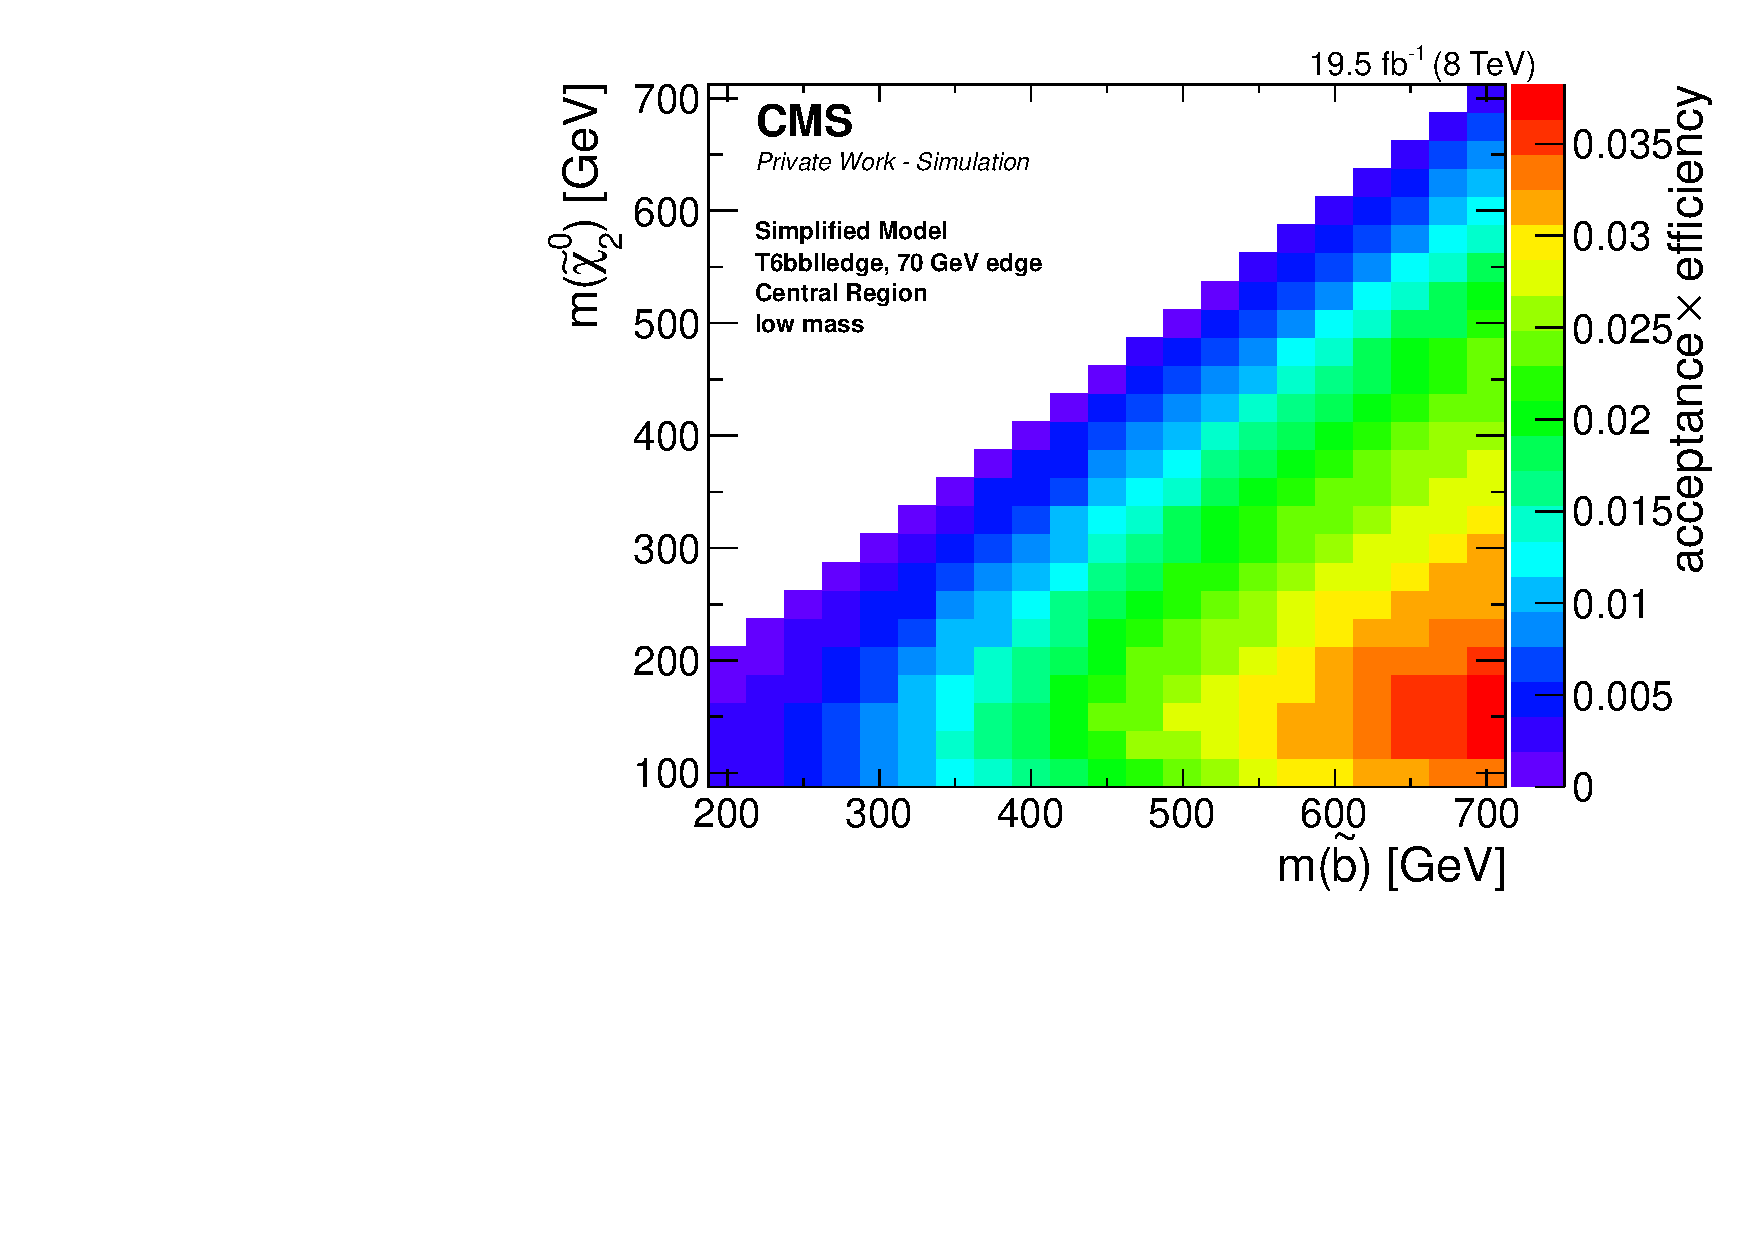
\includegraphics[width=\textwidth]{plots/limits/T6bblledge_70_GeV_Edge_Barrel_lowMll_signalEfficiency.pdf}
\end{minipage}
\begin{minipage}[t]{0.49\textwidth}
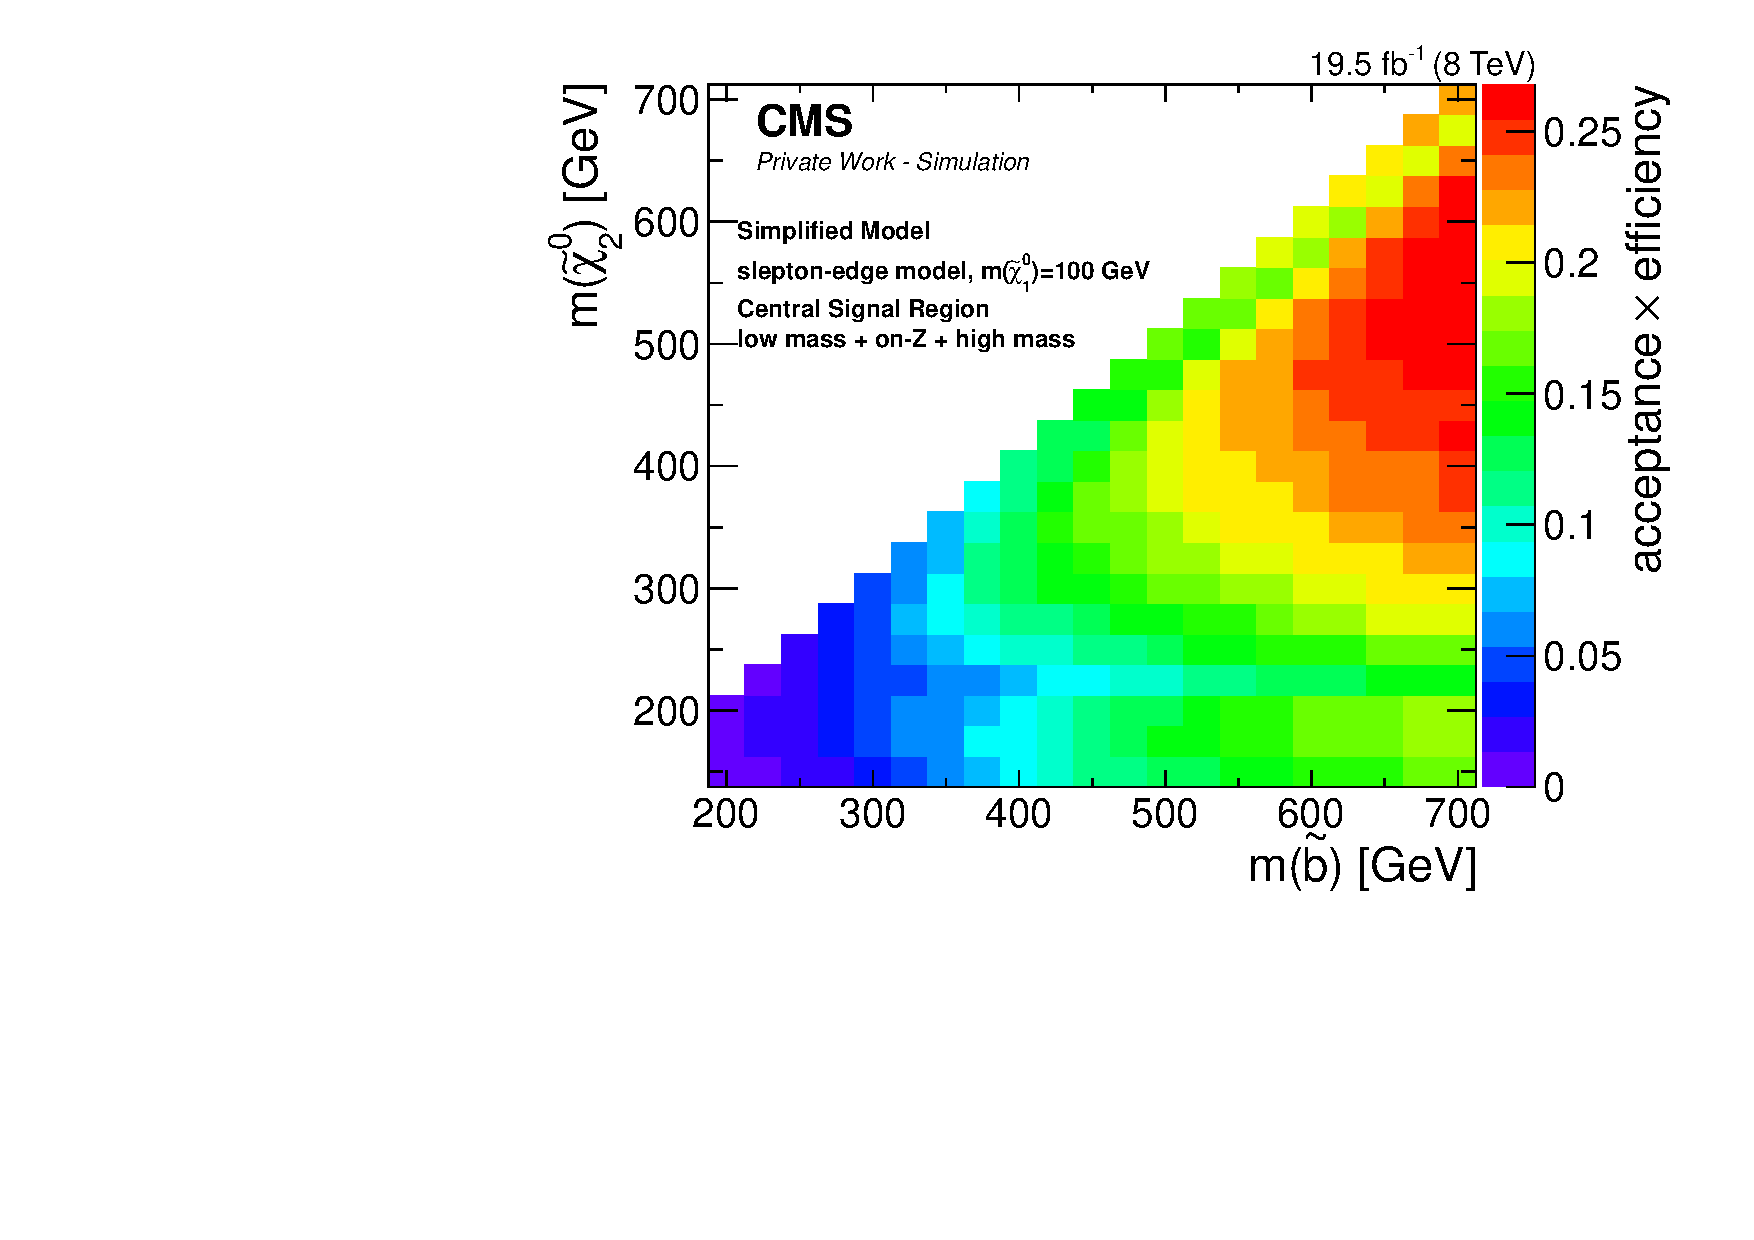
\includegraphics[width=\textwidth]{plots/limits/T6bbllslepton_m_n_1_100_Barrel_signalEfficiency_Reweighted.pdf}
\end{minipage}
\caption{Signal acceptance$\times$efficiency in the $m_{\sbottom}$-$m_{\secondchi}$ plane for the fixed-edge (left) and slepton-edge (right) model for the central signal region.}
\label{fig:sigEff}
\end{figure}
\subsubsection{Systematic uncertainties}
A variety of systematic uncertainties in the signal modelling have to taken into account. The integrated luminosity is measured with a precision of 2.6\%~\cite{CMS-PAS-LUM-13-001}. Variations of the parton distribution functions (PDF) according to the PDF4LHC recommendations~\cite{Alekhin:2011sk,Botje:2011sn,Ball:2012cx,Martin:2009iq,Lai:2010vv} result in an uncertainty of 0--6\% in the signal acceptance. Uncertainties related to lepton efficiencies are of the size of 1\% per lepton. Furthermore, the corrections of the lepton efficiency differences between fast and full detector simulation amount to another 1\% per lepton. The dilepton trigger efficiencies are measured with a precision of 5\%, as described in Section~\ref{sec:triggerEffs}. Uncertainties on the muon momentum scale have negligible impact on the signal acceptance, whereas the uncertainty in the electron energy scale is 0.6\% for central and 1.5\% for forward leptons. Jet energy scale uncertainties~\cite{1748-0221-6-11-P11002} result in an uncertainty in the signal yield of 0--8\%. The uncertainties in the modeling of the objects in the events are propagated to the \MET measurements, resulting in an uncertainty in the signal acceptance of 0--8\%. Here the contributions from the jet energy scale uncertainties are dominant. The events are corrected for difference between observed data and the modelling of initial-state-radiation (ISR) in Madgraph~\cite{Chatrchyan:2013xna} Uncertainties in these corrections are propagated to the event selection and result in an uncertainty of 0--14\% in the signal yield.
The uncertainty associated with pileup reweighting is evaluated by shifting the inelastic cross section by $\pm5\%$, resulting in an uncertainty on the signal acceptance of about 1\%. The uncertainties are summarised in Table~\ref{tab:sysUncerts}.

\begin{table}
\begin{center}
\caption{Summary of systematic uncertainties on the signal efficiency.}
\label{tab:sysUncerts}
\begin{tabular}{l|c}
Uncertainty source & Impact on signal yield [\%]\\ \hline 
Luminosity & 2.6 \\
PDFs on acceptance & 0--6 \\ 
Lepton identification/isolation & 2\\
Fast simulation lepton identification/isolation & 2 \\
Dilepton trigger & 5 \\
Lepton energy scale & 0--5  \\
\MET & 0--8  \\
Jet energy scale/resolution & 0--8  \\
ISR modeling & 0--14 \\
Additional interactions & 1 \\
%\multicolumn{2}{c}{Theoretical Uncertainties}\\
%\hline
%Fact./Renorm. Scale and PDFs& 14-18   \\
\end{tabular}
\end{center}
\end{table}
The combined systematic uncertainties are shown in Figure~\ref{fig:sys}. For the most part of the $m_{\sbottom}$-$m_{\secondchi}$ plane it ranges from 5-7\%. However, close to the diagonal this increases, caused by a larger impact of JES and ISR uncertainties. This is due to the overall lower jet \pt in this region, increasing the probability for threshold effects around the jet \pt requirement of $\unit{40}{\giga\electronvolt}$. The largest uncertainties are observed for both low masses of the \sbottom and \secondchi, exceeding 20\% for the fixed-edge model and   reaching 15\% for the slepton-edge model.
\begin{figure}[htbp]
\centering
\begin{minipage}[t]{0.49\textwidth}
  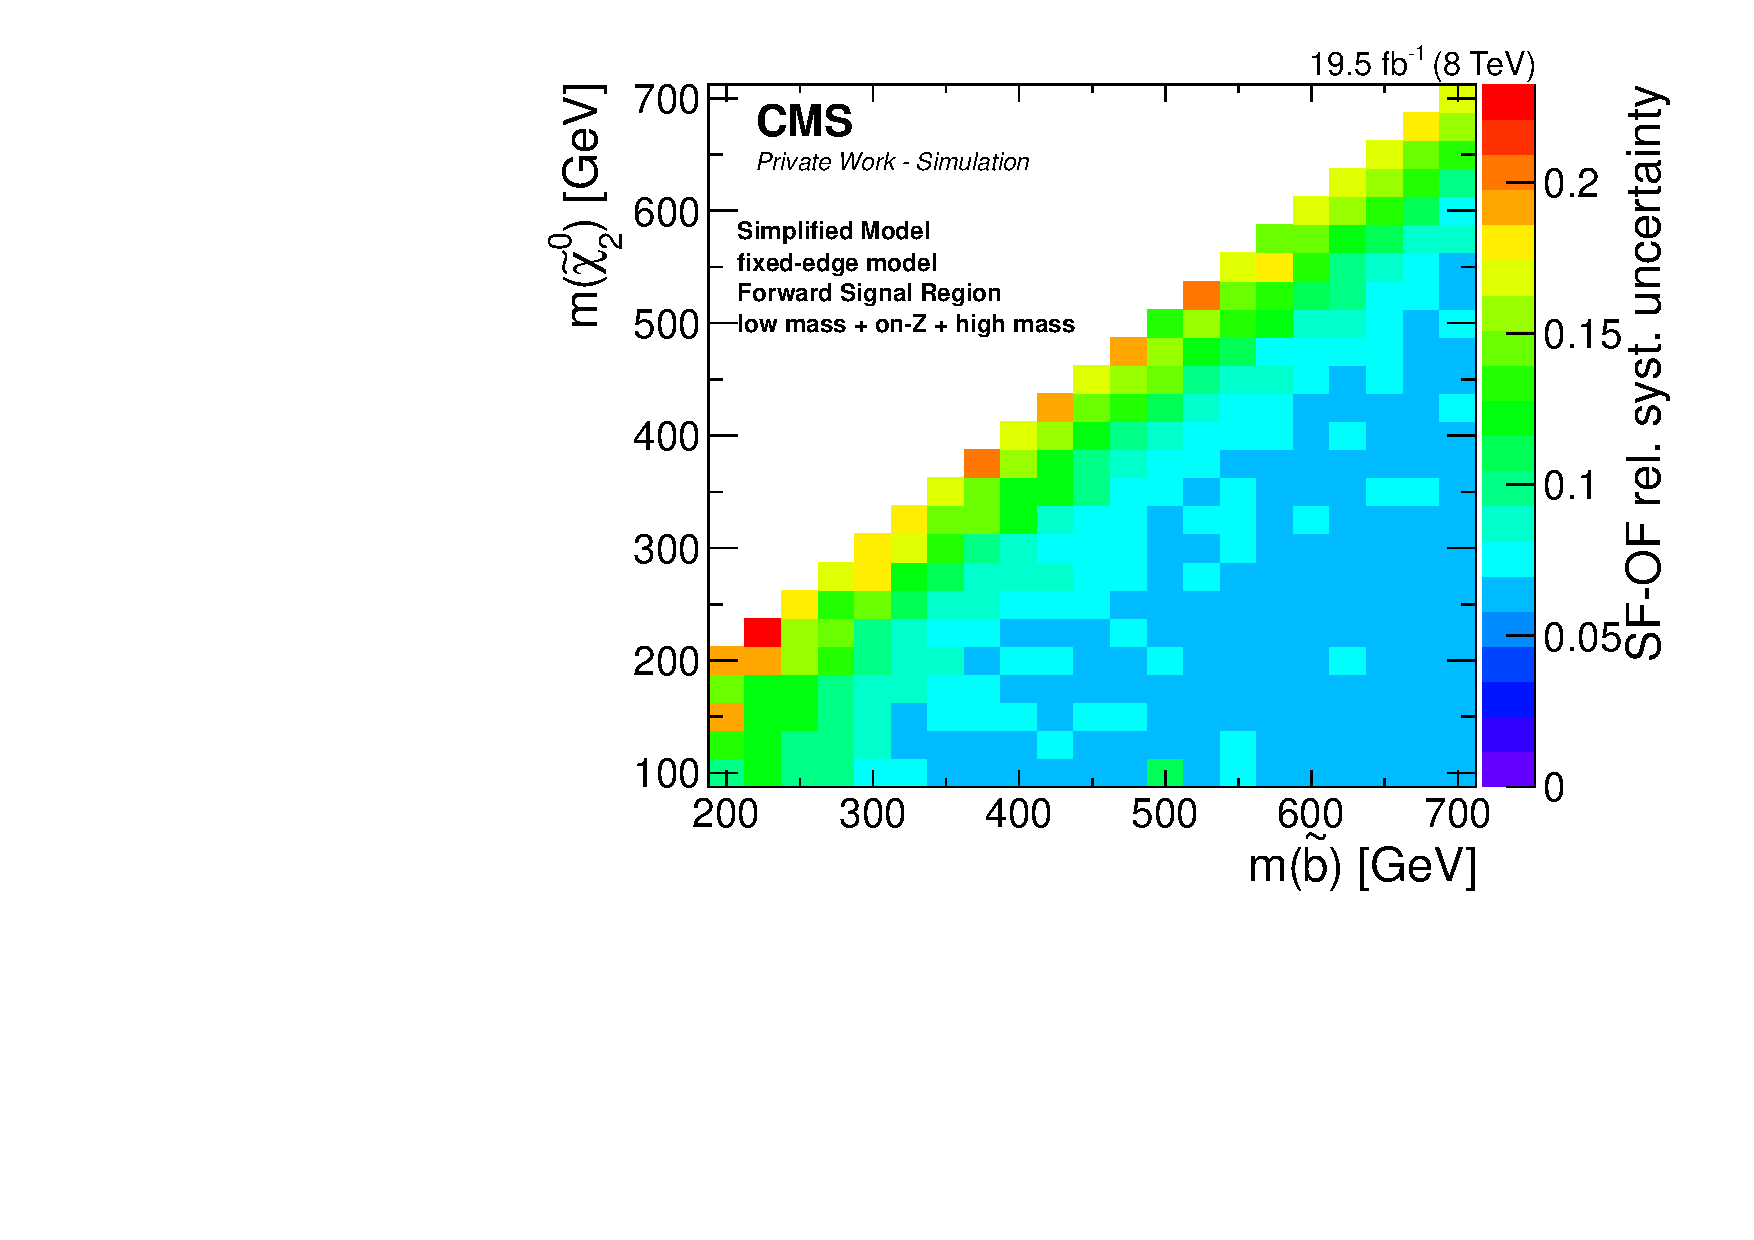
\includegraphics[width=\textwidth]{plots/limits/T6bblledge_70_GeV_Edge_Endcap_syst_err.pdf}
\end{minipage}
\begin{minipage}[t]{0.49\textwidth}
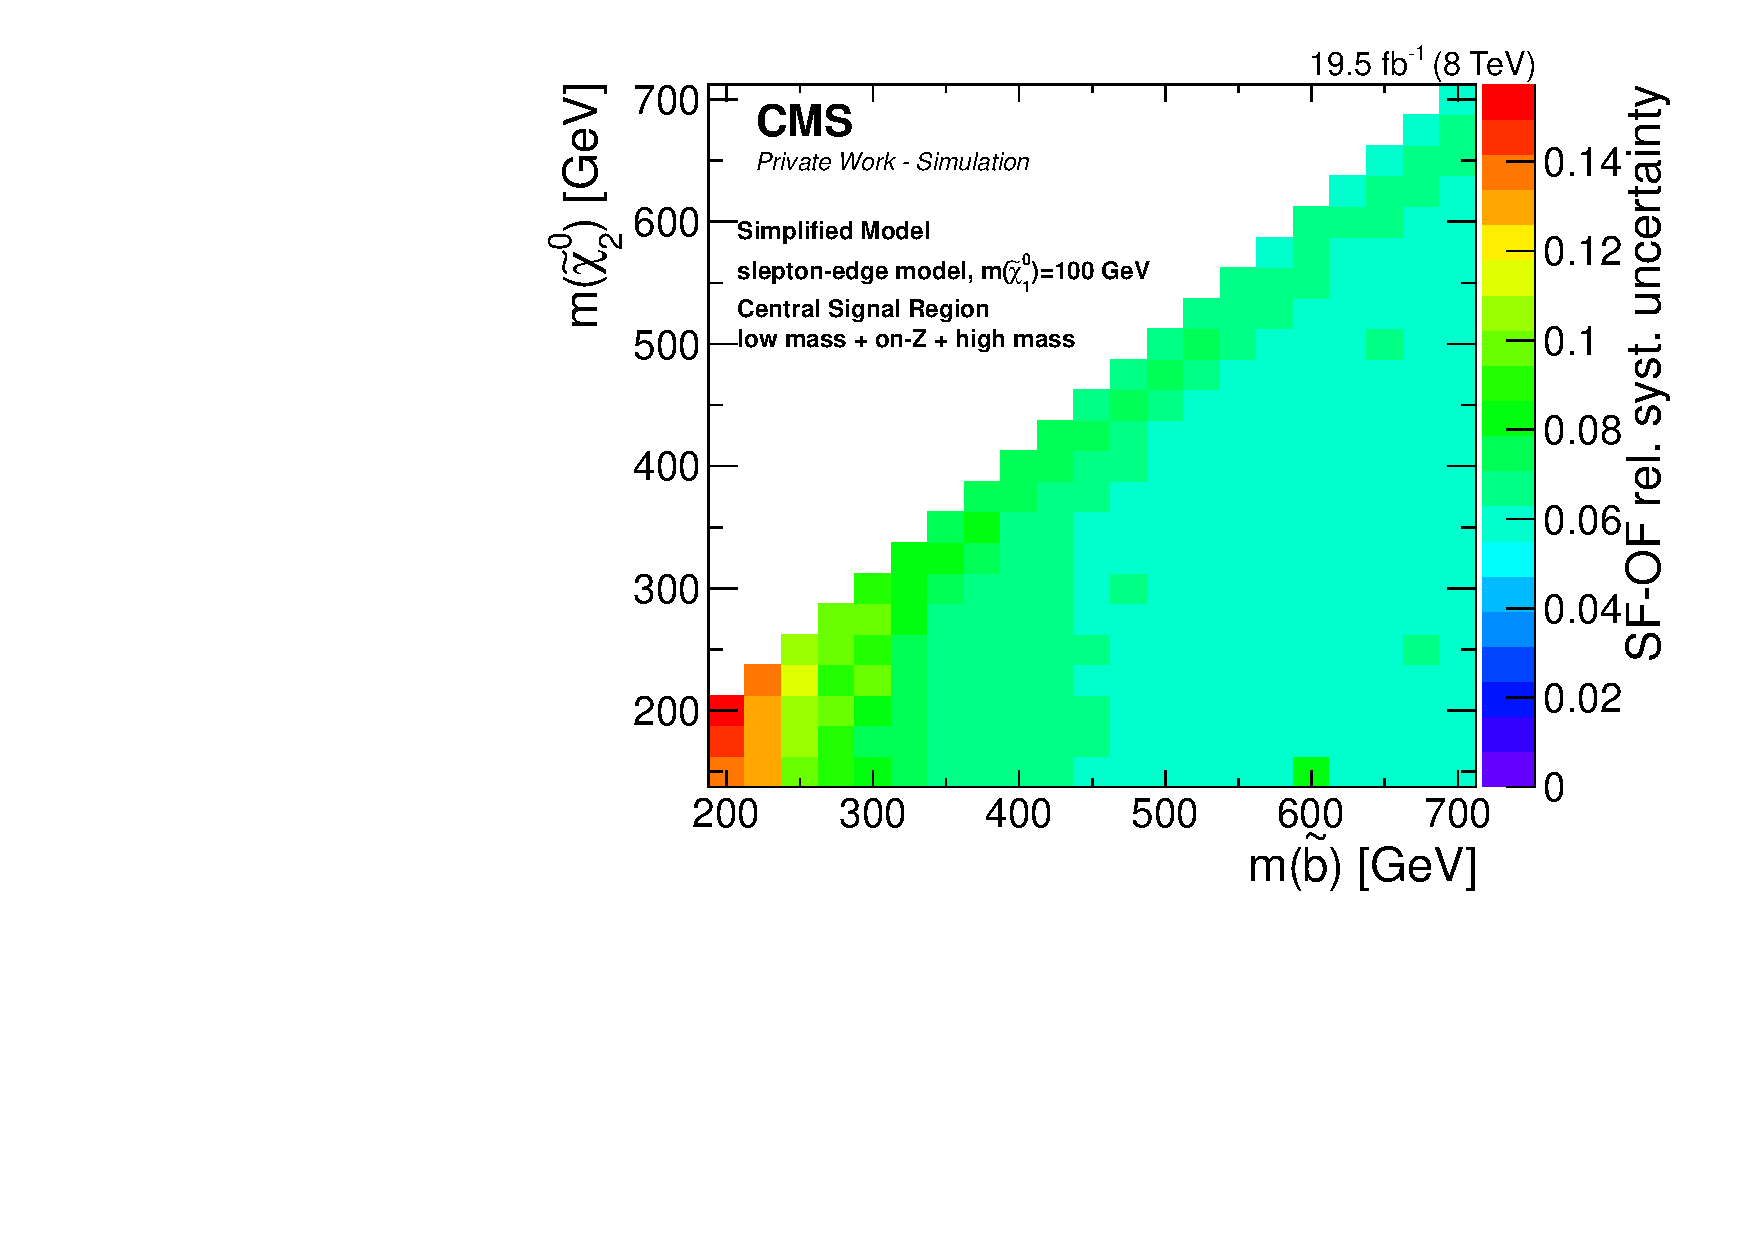
\includegraphics[width=\textwidth]{plots/limits/T6bbllslepton_m_n_1_100_Barrel_syst_err_Reweighted.pdf}
\end{minipage}
\caption{Systematic uncertainty on the signal yield in the central signal region in the $m_{\sbottom}$-$m_{\secondchi}$ plane for the fixed-edge (left) and slepton-edge (right) model.}
\label{fig:sys}
\end{figure}
\subsection{Statistical interpretation}
The results of the counting experiment are translated into exclusion limits by testing the compatibility of the signal plus background ($s+b$) and background only ($b$) hypothesis, treating each signal point in the parameter scans as a separate signal hypothesis. For this purpose, a likelihood function is defined~\cite{HiggsTool1}
\begin{equation}
\label{eq:like}
\mathcal{L}(data|\mu,\theta) = \text{Poisson}(data|\mu\cdot s(\theta) + b(\theta))\cdot p(\tilde{\theta}|\theta),
\end{equation}
where $\mu$ is a signal strength parameter, $\mu = 0$ corresponding to the background only hypothesis and $\mu > 0$ to the  $s+b$ hypothesis, and $p(\tilde{\theta}|\theta)$ parametrises the nuisance parameters $\theta$, with $\tilde{\theta}$ being the nominal value of these parameters. Based on these likelihoods, a test statistic is defined utilizing a profile likelihood ratio: 
\begin{equation}
\tilde{q_{\mu}} = -2 ln\frac{\mathcal{L}(data|\mu,\hat{\theta}_\mu)}{\mathcal{L}(data|\hat{\mu},\hat{\theta})},
\end{equation}
where the $\hat{\theta}_\mu$ represent the maximum likelihood estimators for the nuisance parameters for a given $\mu$, whereas $\hat{\mu}$ and $\hat{\theta}$ indicate the global maximum of the likelihood. For the parametrisation of the nuisance parameters $p(\tilde{\theta}|\theta)$ in equation~\ref{eq:like}, log-normal distributions are chosen. The distribution of the test statistics is then sampled dicing pseudo-experiments for some $\mu > 0$ and $\mu = 0$, representing the $s+b$ and $b$ hypotheses that are tested. The p-values $p_{s+b}$ and $p_{b}$ are defined as the probability to obtain a value of the test statistics as large or larger than the one observed in data for the given hypothesis. To obtain an upper limit on the signal cross section the value of $\mu$ is chosen where $\mathrm{CL}_{\mathrm{s}} = \frac{p_{s+b}}{p_b}$ equals 0.05, corresponding to a 95\% confidence level (CL). In the calculation, all six bins of the counting experiment are combined by multiplying the likelihoods of the different channels. In this procedure, all uncertainties on both background and signal are assumed to be uncorrelated among each other but fully correlated among the different bins.

The resulting exclusion limits are shown in Figure~\ref{fig:limits}. The left plot shows the exclusion limit in the $m_{\sbottom}$-$m_{\secondchi}$ plane for the fixed-edge model. As this model is specifically tuned to provide signals consistent with the excess observed in the low-mass central signal region, the observed limit deviates from the expected one by about $\unit{75}{\giga\electronvolt}$. Given the assumption of this model, \sbottom masses up to about $\unit{375}{\giga\electronvolt}$ are excluded, depending on the mass of the \secondchi. The right plot shows the limit for the slepton-edge model. Because of the much larger branching fraction into leptons in this model, higher masses can be excluded. The expected limit reaches \sbottom masses of about $\unit{600}{\giga\electronvolt}$ roughly independent of $m_{\secondchi}$, except for the region around $m_{\secondchi} = \unit{225}{\giga\electronvolt}$, where it drops below $\unit{550}{\giga\electronvolt}$ because of the gaps in acceptance discussed above. For lower $m_{\secondchi}$ the observed limit is significantly weaker than the expected one as here the limit is dominated by the low-mass signal region in which the excess was observed. For higher $m_{\secondchi}$, the observed limit agrees with the expected one within one standard deviation. The observed lower limit on $m_{\sbottom}$ ranges from $\unit{470}{\giga\electronvolt}$ to $\unit{590}{\giga\electronvolt}$, depending on $m_{\secondchi}$.
\begin{figure}[htbp]
\centering
\begin{minipage}[t]{0.49\textwidth}
  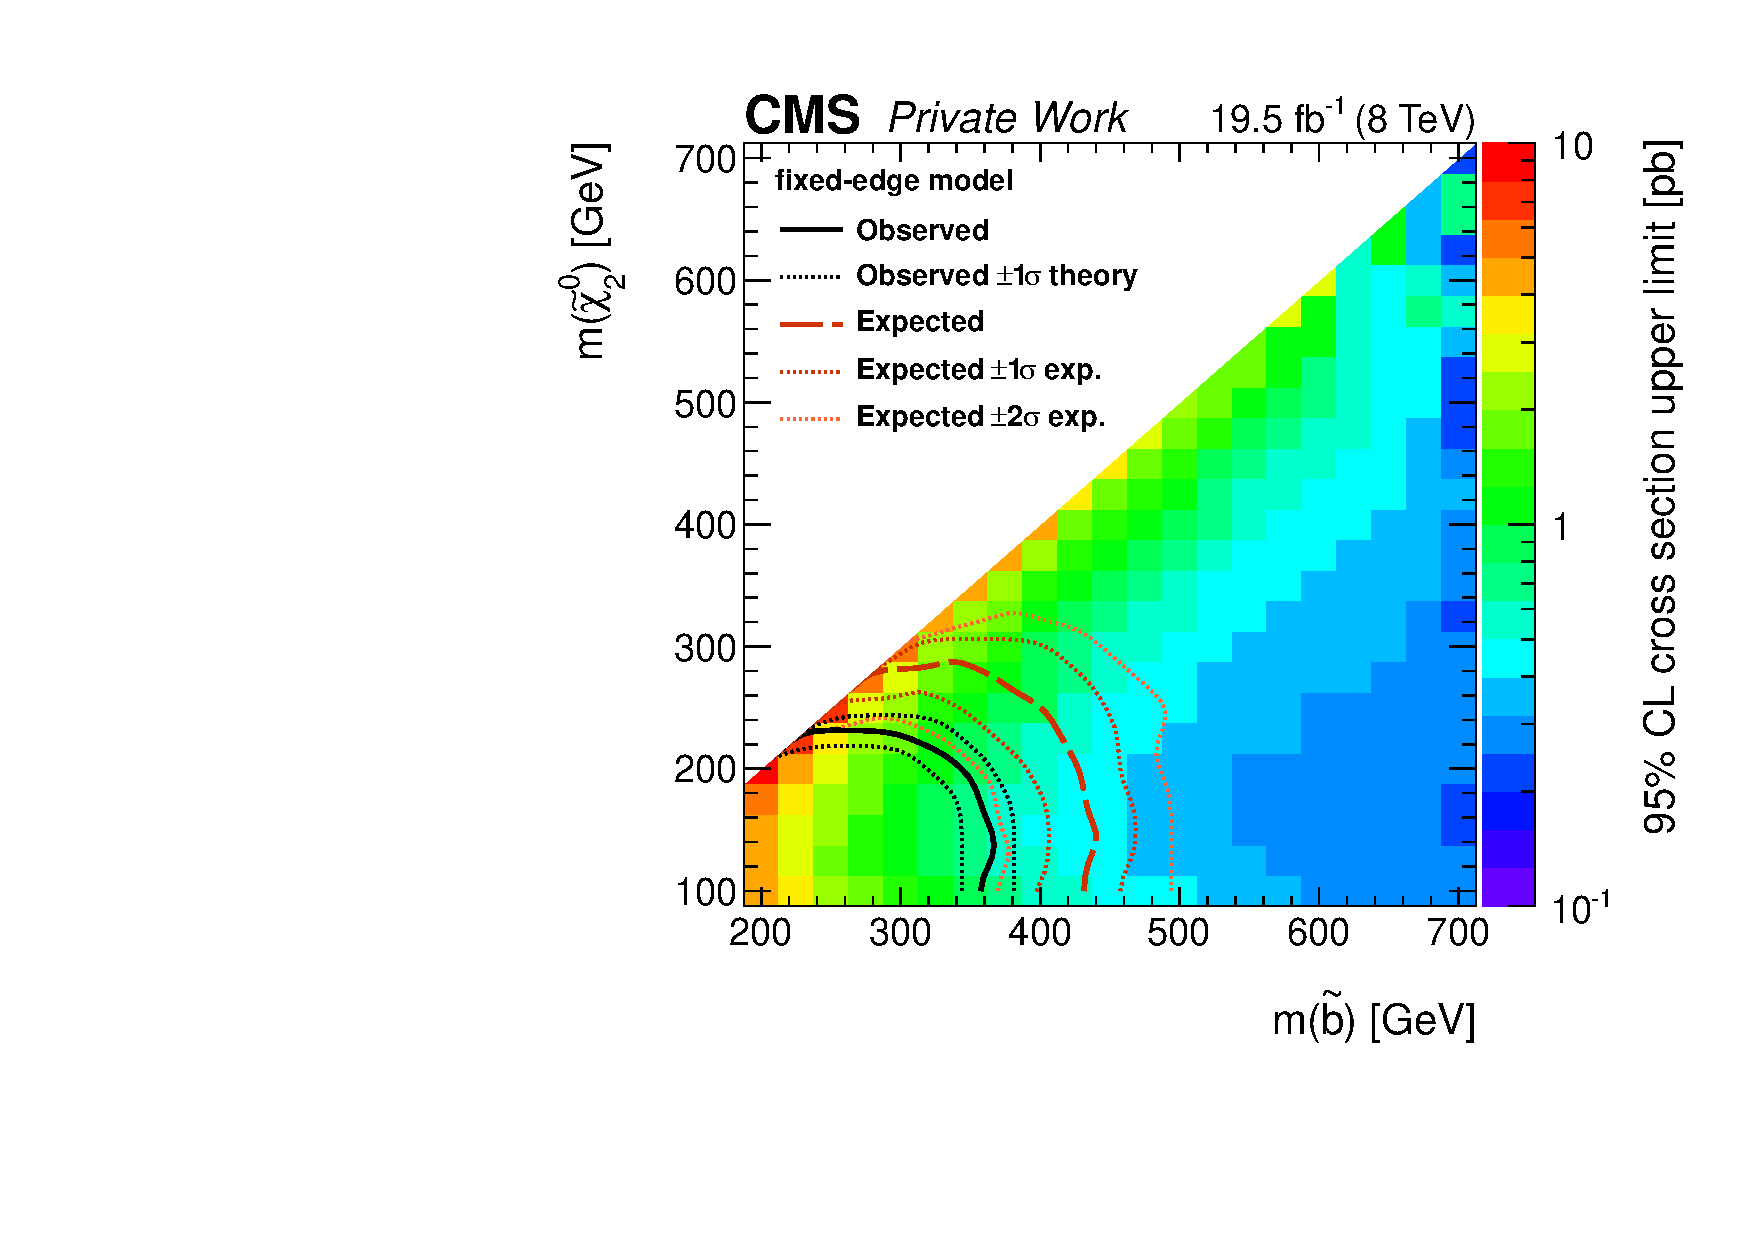
\includegraphics[width=\textwidth]{plots/limits/Fixed_Edge_sbottom_neutralino2_Exclusion_witXsecLimit.pdf}
\end{minipage}
\begin{minipage}[t]{0.49\textwidth}
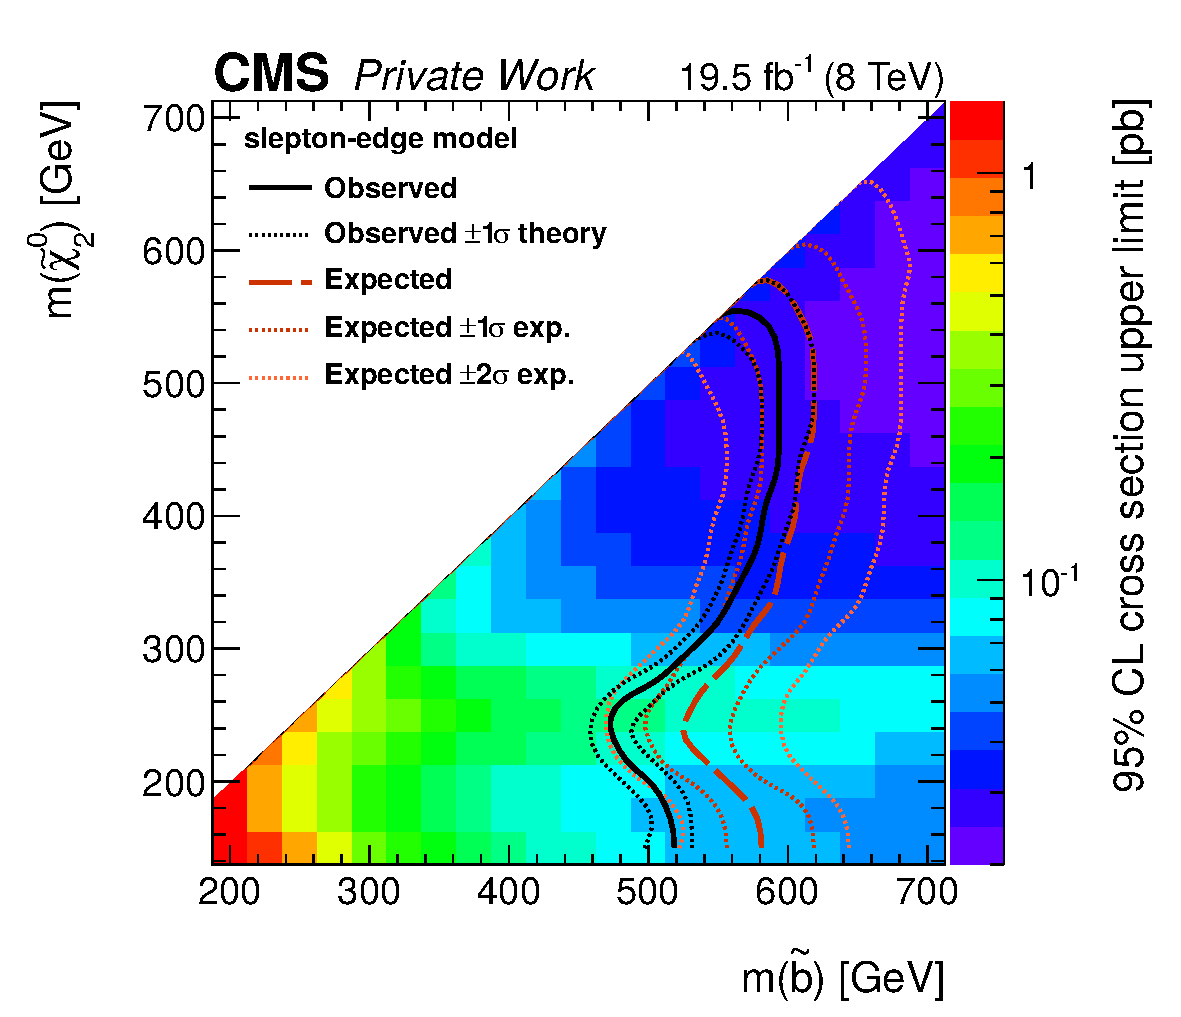
\includegraphics[width=\textwidth]{plots/limits/Fixed_Neutralino_sbottom_neutralino2_Exclusion_witXsecLimit.pdf}
\end{minipage}
\caption{Exclusion limits in the $m_{\sbottom}$-$m_{\secondchi}$ plane for the fixed-edge (left) and slepton-edge (right) model. For each signal point the upper cross section limit is shown colour coded. The intersection of the theoretical with the excluded cross section is shown as a solid black line, with every signal point to the left and below the curve being excluded. The $1-\sigma$ uncertainty interval on the observed limit is shown as dotted black lines. The expected limit together with the $1-$ and $2-\sigma$ interval are shown as brownish solid and dashed lines.}
\label{fig:limits}
\end{figure}